\documentclass[11pt,a4paper]{article}

\usepackage[a4paper,top=22mm,bottom=24mm,left=22mm,right=22mm,headheight=15pt]{geometry}
\usepackage[T1]{fontenc}
\usepackage[utf8]{inputenc}
\usepackage{lmodern}
\usepackage{microtype}
\usepackage{amsmath,amssymb,bm,mathtools}
\usepackage{booktabs,tabularx,longtable,array,multirow}
\usepackage{graphicx}
\usepackage{xcolor}
\usepackage{tikz}
\usetikzlibrary{arrows.meta,positioning,fit,calc,shapes.geometric,backgrounds}
\usepackage[most]{tcolorbox}
\usepackage{enumitem}
\usepackage{caption,subcaption}
\usepackage{fancyhdr}
\usepackage{titlesec}
\usepackage[numbers,sort&compress]{natbib}
\usepackage{hyperref}
\usepackage[nameinlink,noabbrev]{cleveref}

\definecolor{navy}{HTML}{15324A}
\definecolor{blue}{HTML}{1E6A8D}
\definecolor{cyan}{HTML}{58AFC4}
\definecolor{teal}{HTML}{24837B}
\definecolor{orange}{HTML}{D47A32}
\definecolor{red}{HTML}{B94B50}
\definecolor{ink}{HTML}{263238}
\definecolor{muted}{HTML}{60747D}
\definecolor{paper}{HTML}{F5F8F9}
\definecolor{pale}{HTML}{EAF2F5}
\definecolor{greenpale}{HTML}{E8F3EE}
\definecolor{orangepale}{HTML}{FAEFE5}

\hypersetup{
  colorlinks=true,
  linkcolor=navy,
  citecolor=teal,
  urlcolor=blue,
  pdftitle={Online Visuo-Proprioceptive Contact-Response Fields for Physically Coupled Quadruped Digital Twins},
  pdfauthor={Krishna Karthikeya G. N.}
}

\pagestyle{fancy}
\fancyhf{}
\fancyhead[L]{\small\color{muted}UGP Research Proposal}
\fancyhead[R]{\small\color{muted}Visuo-Proprioceptive Contact-Response Fields}
\fancyfoot[C]{\small\color{muted}\thepage}
\renewcommand{\headrulewidth}{0.3pt}
\renewcommand{\footrulewidth}{0pt}

\titleformat{\section}{\Large\bfseries\color{navy}}{\thesection}{0.7em}{}
\titleformat{\subsection}{\large\bfseries\color{navy}}{\thesubsection}{0.6em}{}
\titleformat{\subsubsection}{\normalsize\bfseries\color{ink}}{\thesubsubsection}{0.5em}{}
\titlespacing*{\section}{0pt}{2.0ex plus 0.5ex}{0.8ex}
\titlespacing*{\subsection}{0pt}{1.5ex plus 0.4ex}{0.6ex}
\setlist{nosep,leftmargin=1.6em}
\setlength{\parindent}{0pt}
\setlength{\parskip}{0.55em}
\setlength{\tabcolsep}{5pt}
\renewcommand{\arraystretch}{1.15}

\newcommand{\R}{\mathbb{R}}
\newcommand{\E}{\mathbb{E}}
\newcommand{\V}{\mathbb{V}}
\newcommand{\N}{\mathcal{N}}
\newcommand{\M}{\mathcal{M}}
\newcommand{\C}{\mathcal{C}}
\newcommand{\D}{\mathcal{D}}
\newcommand{\T}{\mathcal{T}}
\newcommand{\Lcal}{\mathcal{L}}
\newcommand{\etal}{\textit{et al.}}
\newcommand{\risk}{\operatorname{CVaR}}
\newcommand{\diag}{\operatorname{diag}}
\newcommand{\proj}{\operatorname{proj}}
\newcommand{\softplus}{\operatorname{softplus}}

\newcolumntype{Y}{>{\raggedright\arraybackslash}X}
\newcolumntype{C}[1]{>{\centering\arraybackslash}p{#1}}
\newcolumntype{L}[1]{>{\raggedright\arraybackslash}p{#1}}

\tcbset{
  enhanced,
  boxrule=0.6pt,
  arc=2mm,
  left=2.2mm,right=2.2mm,top=1.5mm,bottom=1.5mm,
  before skip=7pt,after skip=7pt
}
\newtcolorbox{keybox}[1][]{colback=pale,colframe=blue,title=#1,fonttitle=\bfseries\color{navy}}
\newtcolorbox{claimbox}[1][]{colback=greenpale,colframe=teal,title=#1,fonttitle=\bfseries\color{navy}}
\newtcolorbox{warningbox}[1][]{colback=orangepale,colframe=orange,title=#1,fonttitle=\bfseries\color{navy}}

\tikzset{
  block/.style={draw=blue,rounded corners=2mm,fill=pale,thick,align=center,minimum height=9mm,text width=31mm,font=\small},
  physics/.style={draw=teal,rounded corners=2mm,fill=greenpale,thick,align=center,minimum height=9mm,text width=34mm,font=\small},
  decision/.style={draw=orange,rounded corners=2mm,fill=orangepale,thick,align=center,minimum height=9mm,text width=34mm,font=\small},
  arrow/.style={-{Latex[length=2.2mm]},thick,draw=muted},
  feedback/.style={-{Latex[length=2.2mm]},thick,dashed,draw=orange}
}

\begin{document}
\hypersetup{pageanchor=false}

\begin{titlepage}
\thispagestyle{empty}

\begin{tikzpicture}[remember picture,overlay]
  \fill[paper] (current page.south west) rectangle (current page.north east);
  \fill[navy] (current page.north west) rectangle ([yshift=-104mm]current page.north east);
  \fill[cyan] ([yshift=-104mm]current page.north west) rectangle ([yshift=-107mm]current page.north east);
  \draw[teal,line width=1.2pt] ([xshift=22mm,yshift=23mm]current page.south west) -- ([xshift=-22mm,yshift=23mm]current page.south east);
\end{tikzpicture}

\vspace*{10mm}
{\Large\color{cyan}\bfseries UNDERGRADUATE PROJECT PROPOSAL\par}
\vspace{10mm}
{\fontsize{27}{32}\selectfont\color{white}\bfseries
Online Visuo-Proprioceptive\\[2mm]
Contact-Response Fields\par}
\vspace{4mm}
{\Large\color{white}
for Physically Coupled Quadruped Digital Twins\par}

\vspace{28mm}
\begin{tcolorbox}[colback=paper,colframe=blue,width=\textwidth,boxrule=0.9pt,arc=3mm]
\textbf{Research objective.} Learn a local, uncertainty-aware foot--terrain interaction law from controlled single-leg experiments; attach it to a registered terrain twin; fuse local observations into a persistent world map; compose four shared contact laws through floating-base dynamics; and select globally valid, locally safe actions before the quadruped reaches unseen terrain.
\end{tcolorbox}

\vfill
\begin{tabularx}{\textwidth}{@{}lY@{}}
\textbf{Prepared by} & Krishna Karthikeya G. N.\\
\textbf{Roll number} & 250564\\
\textbf{Document type} & Detailed six-month UGP research and execution plan\\
\textbf{Prepared for} & Mentor review and project approval\\
\textbf{Date} & August 2026\\
\end{tabularx}

\vspace{14mm}
{\small\color{muted}
Scope discipline: the core contribution is the learned contact law and its validated composition. Photorealistic reconstruction, online adaptation, and risk-aware planning are built around that core in staged, falsifiable increments.\par}
\end{titlepage}

\hypersetup{pageanchor=true}
\pagenumbering{roman}

\begin{abstract}
Quadruped navigation systems can often recognize terrain appearance or learn an end-to-end forward model, yet they rarely expose a physically composable account of what each foot will experience. This proposal develops an \emph{online visuo-proprioceptive contact-response field}: a spatial field whose visual and geometric observations index a probabilistic local foot--terrain law, rather than a terrain label or a single nominal friction coefficient. The law predicts three-dimensional ground-reaction force from foot state, penetration, slip velocity, commanded loading, and recurrent terrain state. Four shared copies are coupled through standard floating-base multibody dynamics, producing whole-body motion under candidate control sequences. A photorealistic renderer and a collision/height representation are registered in the same world frame so that a future foothold queries the correct appearance, geometry, contact posterior, and uncertainty. Local observations are fused into a persistent occupancy--geometry--physical map; A*/D* Lite supplies a globally valid route around concave obstacles, while local MPPI evaluates short-horizon physical safety. Once a foothold is touched, proprioceptive and force evidence update only its low-dimensional physical posterior and a sparse residual memory; the visual backbone is not fine-tuned online.

The project is deliberately staged. Real measurements first validate the single-leg law; only then is four-leg composition evaluated in simulation and, subject to access, with limited safe whole-body trials. The planner uses uncertainty-sampled model-predictive path integral control and a risk-sensitive cost. The central hypothesis is falsifiable: a locally learned contact law, trained over the quadruped operating envelope and separated from actuator error, should predict unseen full-body response better than uniform-contact simulation, visual-only parameter prediction, or black-box forward dynamics, while providing calibrated uncertainty. The document specifies equations, instrumentation, dataset design, neural architecture, training losses, online Bayesian fusion, simulator integration, planning, baselines, ablations, acceptance criteria, risks, deliverables, and a 26-week execution schedule.
\end{abstract}

\begin{keybox}[One-sentence thesis]
\textbf{Appearance plus geometry predicts a distribution over local contact dynamics; rigid-body mechanics composes those dynamics into action-conditioned whole-body response; real contact closes the loop by correcting the local posterior.}
\end{keybox}

\tableofcontents
\clearpage
\listoffigures
\listoftables
\clearpage

\pagenumbering{arabic}

\section{Problem Definition and Research Positioning}
\label{sec:problem}

\subsection{The gap}

A quadruped approaching an untouched patch of ground must answer a counterfactual question: \emph{what will happen to the body if a particular foot lands here under a particular gait and command?} A semantic label such as ``grass'' is insufficient. Visually similar grass can be dry or waterlogged; visually different surfaces can have the same mechanical response. Conversely, a single scalar ``traversability'' score cannot distinguish between lateral slip, vertical collapse, impact, actuator saturation, or a transient loss of velocity tracking.

Perception-conditioned forward models already predict platform motion or failure directly from exteroception, proprioceptive history, and candidate actions \citep{roth2025perceptive,kim2022forward}. Vision-to-physics systems infer simulator parameters such as friction and stiffness \citep{chen2024terrain}, while uncertainty-aware traversability estimators improve behavior on out-of-distribution terrain \citep{cai2024pietra,ren2024topnav,zhang2024traversability}. Real-to-sim methods align visual reconstruction and collision geometry \citep{chen2026quadverse,escontrela2025gaussgym,han2025re3sim}, and neural time fields solve Eikonal-style planning problems \citep{ni2023ntfields,liu2025active}. Each ingredient is useful, but their combination leaves an important missing link:

\begin{claimbox}[Research gap]
Existing work does not yet provide a compact, experimentally identified \textbf{local foot--terrain law} that is (i) indexed by registered visual and geometric evidence, (ii) conditioned on the actual contact state and loading, (iii) composable across four feet through explicit multibody mechanics, (iv) updated online after contact, and (v) validated against real force and motion rather than treated as a simulator label.
\end{claimbox}

The original intuition ``change in visual feature $\Delta z$ maps to change in proprioception $\Delta p$'' is therefore refined. That direct mapping is generally ill-posed because the response also depends on the robot state, action, contact mode, geometry, and history. The proposed causal chain is
\begin{equation}
\underbrace{(z_\xi,g_\xi)}_{\text{pre-contact evidence}}
\longrightarrow
\underbrace{q(\eta_\xi,\ell_\xi)}_{\text{contact-law posterior}}
\xrightarrow[\text{action }U]{\text{four-leg dynamics}}
\underbrace{q(X_{t+1:t+H},R_{t+1:t+H})}_{\text{response and risk}},
\label{eq:causal_chain}
\end{equation}
where $\xi$ is a terrain cell, $z_\xi$ a visual embedding, $g_\xi$ local geometry, $\eta_\xi$ interpretable effective parameters, $\ell_\xi$ a residual latent variable, $U$ a candidate command sequence, and $R$ a set of risk observables.

\subsection{Research question, hypotheses, and contribution}

\begin{keybox}[Primary research question]
Can local foot--terrain interaction laws learned from controlled single-leg trials be composed through floating-base multi-contact dynamics to predict full-body quadruped response on visually observed but untouched terrain, using sparse real interactions and calibrated uncertainty?
\end{keybox}

The proposal tests four linked hypotheses.

\begin{table}[ht]
\centering
\caption{Falsifiable hypotheses. Targets are pre-registration goals and will be adjusted only if the measured sensor noise floor makes them physically unattainable.}
\label{tab:hypotheses}
\begin{tabularx}{\textwidth}{@{}C{9mm}Y Y@{}}
\toprule
 & \textbf{Hypothesis} & \textbf{Evidence required}\\
\midrule
H1 & A physics-guided residual contact model predicts held-out three-axis contact force and impulse better than a uniform analytical contact model. & Held-out terrain/condition force NRMSE, impulse error, slip-onset classification, and calibrated intervals.\\
H2 & Four shared copies of the single-leg law, coupled through multibody dynamics, improve short-horizon body-response prediction without retraining an unconstrained whole-robot model. & Base velocity/orientation, joint state, contact timing, and rollout error under unseen load distributions and gaits.\\
H3 & A visual--geometric prior can predict the post-contact physical posterior before touch, while correctly increasing uncertainty for ambiguous or out-of-distribution appearance. & Leave-one-terrain-family-out NLL, interval coverage, risk calibration, and adaptation curves after one to five contacts.\\
H4 & Uncertainty-aware rollouts reduce slip, instability, and failed traversal relative to deterministic or visual-only baselines at comparable progress. & Success, fall/stall rate, slip distance, CVaR cost, time, and energy over repeated trials.\\
H5 & Persistent world-frame mapping plus incremental global route search avoids concave-obstacle local minima that trap robot-centric greedy waypoint selection. & U-shape/cul-de-sac escape success, collision/stall rate, replanning latency, and path ratio to a known-map optimum.\\
\bottomrule
\end{tabularx}
\end{table}

The intended contribution is a \emph{method and validation protocol}, not merely a larger network:
\begin{enumerate}
  \item a constrained three-dimensional contact law with a recurrent terrain state and a small learned residual;
  \item a disciplined single-leg-to-four-leg composition procedure that separates actuator error from terrain error;
  \item a registered visual--geometric--physical terrain field and a cross-modal teacher--student model for pre-contact inference;
  \item an online low-dimensional posterior update with explicit uncertainty and a hierarchical interface to persistent global mapping, D* Lite route search, and local risk-aware planning; and
  \item a dataset, contact and U-shape benchmarks, baselines, ablations, and acceptance gates that make each claim falsifiable.
\end{enumerate}

\subsection{What is novel, reused, and deliberately out of scope}

\begin{table}[ht]
\centering
\caption{Positioning against the closest methodological families.}
\label{tab:positioning}
\small
\begin{tabularx}{\textwidth}{@{}L{31mm}Y Y@{}}
\toprule
\textbf{Family} & \textbf{What is reused} & \textbf{What this proposal adds}\\
\midrule
Perceptive forward dynamics \citep{roth2025perceptive,kim2022forward} & Action-conditioned rollout prediction and sampling-based local planning. & A per-foot contact interface constrained by force mechanics, enabling composition, local correction, and physical diagnosis.\\
Vision-to-physics \citep{chen2024terrain} & Cross-modal visual prediction of effective simulator quantities. & Real force supervision, recurrent/deformable state, posterior rather than point estimate, and explicit distinction between effective parameters and material truth.\\
Evidential traversability \citep{cai2024pietra,ren2024topnav} & OOD-aware risk and proprioceptive correction. & Correction of a spatial contact-law posterior that is rolled through full-body dynamics, rather than correction of a terrain class or scalar score.\\
Visual--physical real-to-sim \citep{chen2026quadverse,escontrela2025gaussgym,han2025re3sim} & Registered neural rendering and collision geometry; residual dynamics calibration. & A spatially varying, contact-conditioned, online-updated physical field learned from controlled real interaction.\\
Digital double \citep{haddeler2022digital} & Real-time comparison between predicted and measured response. & Pre-contact visual priors, per-foot force-level correction, and uncertainty-propagated action selection.\\
Neural Eikonal planning \citep{ni2023ntfields,liu2025active} & Arrival-time fields as a possible global planner. & Risk speed derived from the learned contact response; anisotropy is treated explicitly. This remains a stretch module.\\
\bottomrule
\end{tabularx}
\end{table}

\begin{warningbox}[Claims this project will not make]
The inferred $\eta$ values are \textbf{effective simulator/contact parameters}, not guaranteed intrinsic material constants. A photorealistic rendering is not evidence of physical fidelity. Single-leg validation alone does not prove whole-quadruped real-world fidelity. The project does not learn the robot's entire dynamics end-to-end, replace the low-level locomotion controller, or promise general operation on arbitrary mud without reproducible training and validation conditions.
\end{warningbox}

\subsection{System overview}

\Cref{fig:pipeline} shows the contact-response and local-control loop. The persistent global mapping and route-selection layer is specified separately in \cref{fig:global_hierarchy}. Four separations are fundamental: (i) visual prediction is separated from real post-contact evidence; (ii) contact physics is separated from actuator dynamics; (iii) photorealistic rendering is separated from collision geometry while both remain registered; and (iv) global topological route selection is separated from local physical action selection.

\begin{figure}[p]
\centering
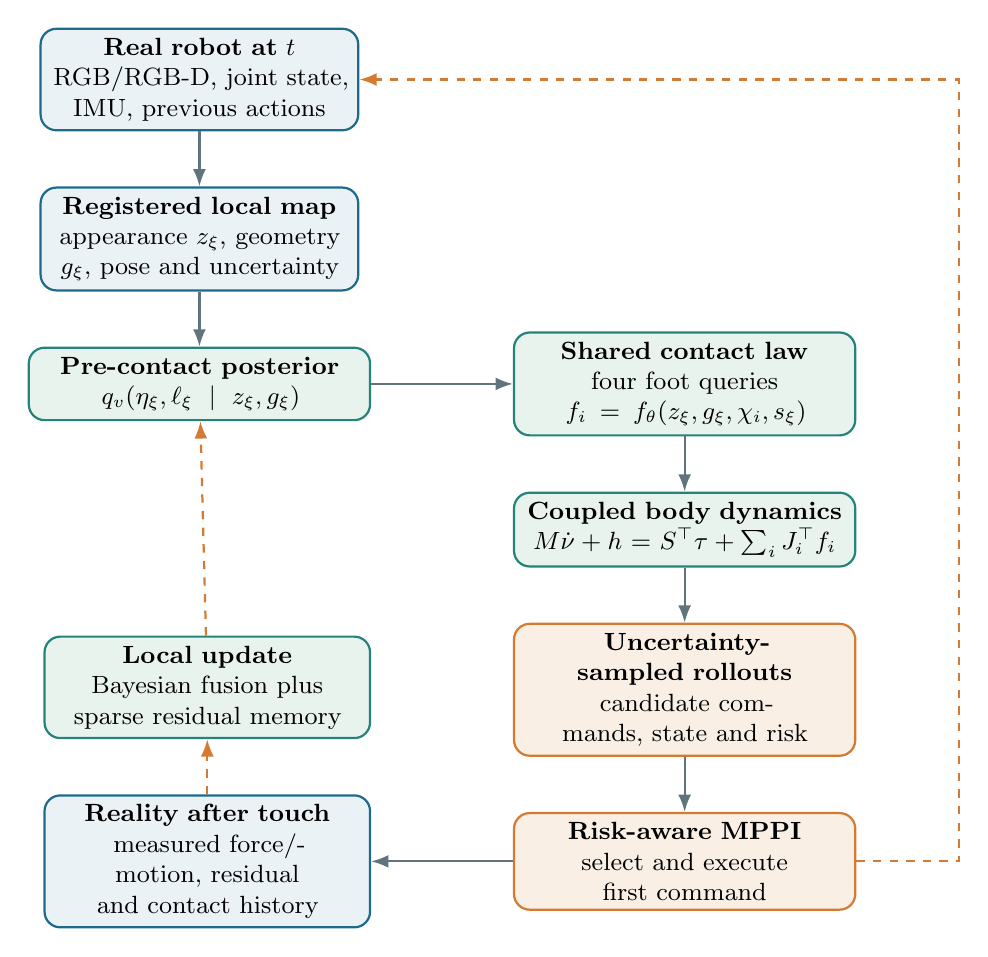
\begin{tikzpicture}[node distance=7mm and 10mm]
  \node[block,text width=38mm] (sense) {\textbf{Real robot at $t$}\\RGB/RGB-D, joint state, IMU, previous actions};
  \node[block,text width=38mm,below=of sense] (map) {\textbf{Registered local map}\\appearance $z_\xi$, geometry $g_\xi$, pose and uncertainty};
  \node[physics,text width=41mm,below=of map] (prior) {\textbf{Pre-contact posterior}\\$q_v(\eta_\xi,\ell_\xi\mid z_\xi,g_\xi)$};

  \node[physics,text width=41mm,right=18mm of prior] (contacts) {\textbf{Shared contact law}\\four foot queries $f_i=f_\theta(z_\xi,g_\xi,\chi_i,s_\xi)$};
  \node[physics,text width=41mm,below=of contacts] (dynamics) {\textbf{Coupled body dynamics}\\$M\dot\nu+h=S^\top\tau+\sum_iJ_i^\top f_i$};
  \node[decision,text width=41mm,below=of dynamics] (rollout) {\textbf{Uncertainty-sampled rollouts}\\candidate commands, state and risk};
  \node[decision,text width=41mm,below=of rollout] (mppi) {\textbf{Risk-aware MPPI}\\select and execute first command};

  \node[block,text width=39mm,left=18mm of mppi] (evidence) {\textbf{Reality after touch}\\measured force/motion, residual and contact history};
  \node[physics,text width=39mm,above=of evidence] (update) {\textbf{Local update}\\Bayesian fusion plus sparse residual memory};

  \draw[arrow] (sense) -- (map);
  \draw[arrow] (map) -- (prior);
  \draw[arrow] (prior) -- (contacts);
  \draw[arrow] (contacts) -- (dynamics);
  \draw[arrow] (dynamics) -- (rollout);
  \draw[arrow] (rollout) -- (mppi);
  \draw[arrow] (mppi) -- (evidence);
  \draw[feedback] (evidence) -- (update);
  \draw[feedback] (update) -- (prior);
  \draw[feedback] (mppi.east) -- ++(13mm,0) |- (sense.east);
\end{tikzpicture}
\caption{Contact-response and local-control loop. Untouched terrain is represented by a visual--geometric prior. Candidate actions are evaluated only after the per-foot laws are coupled through mechanics. Real post-contact evidence updates the local field; persistent global route selection is shown in \cref{fig:global_hierarchy}.}
\label{fig:pipeline}
\end{figure}

\subsection{Notation and operational assumptions}

\begin{table}[ht]
\centering
\caption{Core notation.}
\label{tab:notation}
\small
\begin{tabularx}{\textwidth}{@{}L{20mm}Y L{22mm}Y@{}}
\toprule
\textbf{Symbol} & \textbf{Meaning} & \textbf{Symbol} & \textbf{Meaning}\\
\midrule
$q,\nu$ & Floating-base configuration and generalized velocity & $x=[q,\nu]$ & Full robot state\\
$i\in\{1,\ldots,4\}$ & Foot index & $\xi$ & Terrain cell/patch under a foot\\
$z_\xi$ & Dense visual embedding & $g_\xi$ & Geometry: height, normal, curvature, roughness\\
$\eta_\xi$ & Positive effective contact parameters & $\ell_\xi$ & Low-dimensional residual contact latent\\
$s_{\xi,t}$ & Recurrent/deformable terrain state & $\chi_{i,t}$ & Foot pose, velocity, penetration, command/load context\\
$f_i\in\R^3$ & Ground-reaction force at foot $i$ & $\tau$ & Actuator torque applied through $S$\\
$U$ & Candidate command sequence & $H$ & Prediction horizon\\
$\mu_\xi,\Sigma_\xi$ & Contact posterior mean/covariance & $R$ & Risk observables: slip, tilt, sinkage, collision\\
$\mathcal G_t$ & Persistent world-frame occupancy/physical map & $P_t^*,p_t^{\mathrm{sub}}$ & Global route and current look-ahead subgoal\\
\bottomrule
\end{tabularx}
\end{table}

The core implementation assumes access to a controlled one-legged rig or simulator, synchronized vision and proprioception, and terrain samples supplied in small reproducible patches. A six-axis foot force/torque sensor or force plate is strongly preferred. The full quadruped is used sparingly for safe validation; the method remains valuable if only simulated four-leg validation is available, but the claims will be correspondingly narrower.

\section{Physical Model: From One Foot to Four Coupled Contacts}
\label{sec:physics}

\subsection{State, frames, and the learned object}

Let the floating-base quadruped configuration be $q=(r_B,R_B,q_j)$ and generalized velocity $\nu=(v_B,\omega_B,\dot q_j)$. World, body, foot, contact, and camera frames are denoted $W,B,F_i,C_i,$ and $C$. The contact frame has $z$-axis equal to the local outward terrain normal $n_\xi$. At time $t$, foot $i$ queries terrain cell $\xi(i,t)$ and forms
\begin{align}
g_\xi &= [h_\xi,n_\xi,\kappa_\xi,\rho_\xi], \\
\chi_{i,t} &= [R^W_{F_i},v^W_{F_i},\delta_{i,t},\dot\delta_{i,t},u_t,\hat N_{i,t},c_{i,t}], \\
y_{i,t} &= [z_\xi,g_\xi,\chi_{i,t},s_{\xi,t}],
\label{eq:contact_input}
\end{align}
where $h$ is height, $\kappa$ curvature, $\rho$ roughness, $\delta$ penetration, $u_t$ the high-level command, $\hat N$ predicted normal load, $c$ a contact-mode indicator, and $s$ a history-dependent terrain state.

The learned object is the local contact function
\begin{equation}
f_i^W=f_\theta(y_{i,t})\in\R^3,
\label{eq:learned_contact}
\end{equation}
not an image-to-force mapping and not a force measured at the hip. The same parameters $\theta$ are shared across all four feet. Leg-specific effects enter through kinematics, foot orientation, actuator state, and loading; foot-specific parameters are introduced only if hardware calibration demonstrates a repeatable asymmetry.

\subsection{Physics-guided contact law}

The model uses a constrained analytical backbone plus a small residual. This provides extrapolation behavior, reduces data demand, and prevents obviously non-physical output. The signed distance of the foot surface from the terrain is $\phi_i(q)$ and
\begin{equation}
\delta_i=[-\phi_i(q)]_+,
\qquad
v_{t,i}=(I-n_\xi n_\xi^\top)v_{F_i},
\qquad
v_{n,i}=n_\xi^\top v_{F_i}.
\label{eq:contact_kinematics}
\end{equation}
The visual--geometric model predicts a posterior over positive effective parameters
\begin{equation}
\eta_\xi=[\mu_\xi,k_\xi,c_\xi,\gamma_\xi]
=\big[\softplus(\tilde\mu),\softplus(\tilde k),\softplus(\tilde c),1+\softplus(\tilde\gamma)\big],
\label{eq:positive_params}
\end{equation}
where $\mu$ is effective friction, $k$ normal stiffness, $c$ normal damping, and $\gamma$ a nonlinear indentation exponent. These are useful contact parameters, not claimed intrinsic material constants \citep{chen2024terrain}.

The analytical normal and tangential components in the contact frame are
\begin{align}
\tilde f_{n,i} &= \left[k_\xi\delta_i^{\gamma_\xi}+c_\xi\delta_i^{\gamma_\xi-1}\dot\delta_i\right]_+, \\
\tilde f_{t,i} &= -\mu_\xi\tilde f_{n,i}
\tanh\!\left(\frac{\lVert v_{t,i}\rVert}{v_s}\right)
\frac{v_{t,i}}{\lVert v_{t,i}\rVert+\epsilon},
\label{eq:analytical_contact}
\end{align}
with smoothing speed $v_s$ and numerical constant $\epsilon$. A residual network $r_\rho$ captures phenomena the backbone cannot express:
\begin{equation}
\Delta f^{C_i}_{i,t}=r_\rho\!\left(z_\xi,g_\xi,\chi_{i,t},s_{\xi,t},\ell_\xi\right),
\qquad \Delta f\in\R^3.
\label{eq:force_residual}
\end{equation}
The final contact force is projected to a friction cone and rotated to the world frame:
\begin{align}
\C(\mu_\xi)&=\{(f_t,f_n): f_n\ge 0,\ \lVert f_t\rVert_2\le\mu_\xi f_n\},\\
f_i^W&=R^W_{C_i}\Pi_{\C(\mu_\xi)}
\left(
\begin{bmatrix}\tilde f_{t,i}\\ \tilde f_{n,i}\end{bmatrix}
+\Delta f^{C_i}_{i,t}
\right).
\label{eq:force_projection}
\end{align}
The projection makes non-negative normal force and bounded tangential force structural properties. A soft projection may be used during training; a hard projection is retained during deployment.

\subsection{History-dependent and deformable terrain}

A memoryless law is adequate for rigid rubber, acrylic, or foam over small deformation, but not for granular or muddy terrain. Repeated loading changes sinkage, compaction, and available shear resistance. Each contacted cell therefore stores a small recurrent state
\begin{equation}
s_{\xi,t+1}=\operatorname{clip}\left[s_{\xi,t}+\Delta t\,g_\varphi\!\left(s_{\xi,t},\tilde f_{n,i},\lVert v_{t,i}\rVert,\delta_i,\eta_\xi,\ell_\xi\right)\right],
\label{eq:terrain_state}
\end{equation}
with two to four bounded dimensions interpreted operationally as compaction/sinkage and shear-history state. The update is zero when the cell is not contacted, with an optional slow recovery term. The project will not fit a high-parameter terramechanics model unless the rig excites its parameters independently; an underidentified ``physical'' model is less defensible than a small effective state.

\subsection{Four-foot composition through multibody dynamics}

The quadruped equations are not learned from scratch. Standard rigid-body mechanics couples the four local forces:
\begin{equation}
M(q)\dot\nu+h(q,\nu)=S^\top\tau+\sum_{i=1}^{4}J_i(q)^\top f_i^W+f_{\mathrm{ext}},
\label{eq:rigid_body}
\end{equation}
where $M$ is the mass matrix, $h$ contains Coriolis, centrifugal, and gravity terms, $S$ selects actuated joints, $J_i$ is the foot Jacobian, and $f_{\mathrm{ext}}$ covers known external forces. Four contacts are coupled because every $f_i$ changes base acceleration, joint motion, the load borne by every other leg, and consequently their next contact forces.

\begin{figure}[ht]
\centering
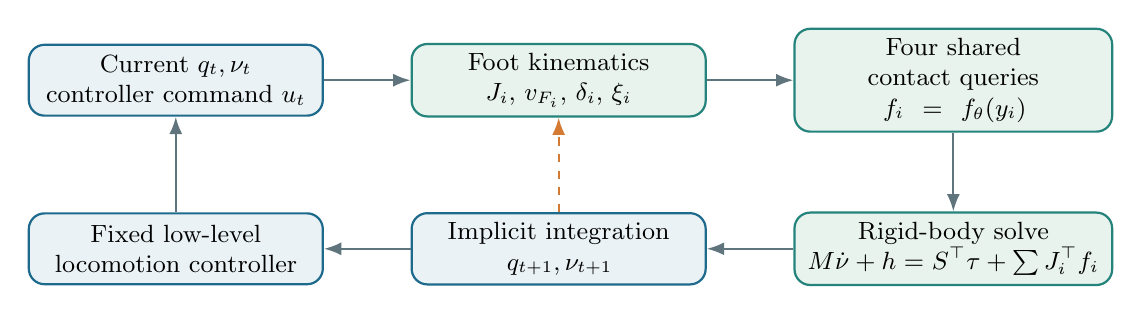
\begin{tikzpicture}[node distance=6mm and 11mm]
  \node[block,text width=35mm] (state) {Current $q_t,\nu_t$\\controller command $u_t$};
  \node[physics,right=of state,text width=35mm] (kin) {Foot kinematics\\$J_i$, $v_{F_i}$, $\delta_i$, $\xi_i$};
  \node[physics,right=of kin,text width=38mm] (forces) {Four shared contact queries\\$f_i=f_\theta(y_i)$};
  \node[physics,below=10mm of forces,text width=38mm] (body) {Rigid-body solve\\$M\dot\nu+h=S^\top\tau+\sum J_i^\top f_i$};
  \node[block,left=of body,text width=35mm] (integrate) {Implicit integration\\$q_{t+1},\nu_{t+1}$};
  \node[block,left=of integrate,text width=35mm] (controller) {Fixed low-level\\locomotion controller};
  \draw[arrow] (state) -- (kin);
  \draw[arrow] (kin) -- (forces);
  \draw[arrow] (forces) -- (body);
  \draw[arrow] (body) -- (integrate);
  \draw[arrow] (integrate) -- (controller);
  \draw[arrow] (controller) -- (state);
  \draw[feedback] (integrate.north) -- ++(0,5mm) -| (kin.south);
\end{tikzpicture}
\caption{The composition claim. No independent ``four-leg network'' is needed for the core model. Whole-body behavior emerges from four state-dependent local forces, a calibrated actuator model, and standard multibody coupling.}
\label{fig:coupling}
\end{figure}

Because force depends on next-step penetration and velocity, an explicit one-pass update may be unstable for stiff contact. The simulator will use semi-implicit/implicit Euler. For a step of duration $\Delta t$,
\begin{equation}
\nu_{t+1}=\nu_t+\Delta t\,M(q_t)^{-1}
\left[S^\top\tau_t-h_t+\sum_iJ_i(q_t)^\top f_i(q_{t+1},\nu_{t+1},s_t)\right].
\label{eq:implicit}
\end{equation}
The contact--load circularity is resolved by the simulator's contact solver or two to five damped fixed-point/Newton iterations. Iteration stops when both generalized-velocity and force changes fall below tolerance. If convergence fails, the step is halved and the rollout is marked high risk. This is critical: the normal load should emerge from the coupled solve, not be supplied as an independent ground-truth input at deployment.

\subsection{Separating actuator error from terrain error}

If motor delay, torque tracking, or joint friction is left unmodelled, the contact network will absorb it and cease to transfer across robots or controllers. Following the residual-dynamics motivation in visually aligned simulators such as QuadVerse \citep{chen2026quadverse}, actuator calibration is performed first on a rigid, high-friction reference floor:
\begin{align}
\tau_t^{\mathrm{real}} &= \tau_t^{\mathrm{nom}}+\Delta\tau_\omega(H_t^a),\\
\tau_t^{\mathrm{nom}} &= K_p(q_t^{\mathrm{des}}-q_t)-K_d\dot q_t+\tau_t^{\mathrm{ff}},
\label{eq:actuator_residual}
\end{align}
where $H_t^a$ contains recent desired/measured joint states, motor current, battery voltage if available, and command history. A small linear time-delay model or two-layer GRU is fitted to rigid-floor trials and then frozen. Terrain experiments subsequently identify $f_\theta$. A final joint fine-tuning stage is permitted only with regularization that preserves the rigid-floor calibration.

\subsection{Single-leg identification: instrumentation and data}

\subsubsection{Minimum instrumentation}

\begin{table}[ht]
\centering
\caption{Recommended sensing and synchronization. Rates are engineering targets, not hard dependencies.}
\label{tab:sensors}
\small
\begin{tabularx}{\textwidth}{@{}L{29mm}L{30mm}Y Y@{}}
\toprule
\textbf{Signal} & \textbf{Target rate} & \textbf{Purpose} & \textbf{Fallback}\\
\midrule
Six-axis foot F/T or force plate & $\ge 500$ Hz & Ground-truth $f^{\mathrm{meas}}$ and impulse & Calibrated inverse dynamics; claims weakened\\
Joint angle/velocity/current or torque & 200--500 Hz & Foot kinematics, actuator model, load context & Encoder differentiation with filtering\\
IMU & $\ge 200$ Hz & Rig/base motion and impact timing & External tracker for constrained rig\\
RGB or RGB-D camera & 20--30 Hz & Appearance, geometry, camera registration & RGB plus measured height/slope\\
Foot/terrain pose or depth & $\ge 100$ Hz & Penetration and local normal & Calibrated kinematics plus static surface scan\\
Hardware timestamps/trigger & common clock & Cross-modal alignment & Offline cross-correlation and clock model\\
\bottomrule
\end{tabularx}
\end{table}

All force labels are expressed at the foot--terrain contact in the local contact frame, then converted to world coordinates using calibrated transforms. A pivot or hip reaction is not used directly as the terrain target. If only actuator torque is available, foot force is inferred by constrained inverse dynamics,
\begin{equation}
J_f(q)^\top \hat f=M_\ell(q)\ddot q+h_\ell(q,\dot q)-\tau-\hat f_{\mathrm{fixture}},
\label{eq:inverse_dynamics_force}
\end{equation}
with acceleration filtering, fixture-force calibration, and uncertainty propagated into the training covariance. This fallback is noisier and may not identify tangential force reliably.

\subsubsection{Excitation protocol}

The dataset must span the operating envelope that a quadruped foot will see. For every terrain patch, the rig performs:
\begin{enumerate}
  \item \textbf{quasi-static indentation} at multiple depths to identify stiffness/nonlinearity;
  \item \textbf{rate sweeps} at multiple vertical speeds to separate damping from stiffness;
  \item \textbf{tangential sweeps} under multiple normal loads and directions to identify friction and anisotropy;
  \item \textbf{combined normal--tangential motion} to expose coupling and slip onset;
  \item \textbf{landing/hopping pulses} to validate impact impulse outside slow identification data; and
  \item \textbf{inclined and repeated contacts} to excite orientation, compaction, and hysteresis.
\end{enumerate}

Core surfaces are chosen to separate mechanical phenomena: rigid high-friction rubber, controlled low-friction acrylic/film, compliant foam, and a reproducible granular/sinkable bed. Mud or wet organic terrain is a final generalization test, not the first training surface. A full factorial design is unnecessary; a D-optimal or Latin-hypercube subset over normal load, vertical speed, tangential speed, inclination, and foot orientation limits collection to approximately 100--150 short episodes per core surface, with at least five repeats at critical boundary conditions.

\subsubsection{Parameter identification and identifiability}

For terrain region $r$, analytical parameters are first identified without a neural residual:
\begin{equation}
\eta_r^*=\arg\min_{\eta}
\sum_{e\in\D_r}\sum_t
\left\lVert f_{e,t}^{\mathrm{meas}}-f_{\mathrm{ana}}(\chi_{e,t};\eta)\right\rVert_{W_f}^2
+\lambda_\eta\lVert\eta-\eta_0\rVert_2^2
+\lambda_E\Lcal_E,
\label{eq:sysid}
\end{equation}
where $\Lcal_E$ penalizes net energy generation over passive contact cycles. A gradient method is used for the differentiable surrogate; grid/Bayesian search is retained for non-differentiable simulator parameters.

Before fitting, local identifiability is checked with the sensitivity/Fisher matrix
\begin{equation}
\mathcal I(\eta)=\sum_{e,t}
\left(\frac{\partial \hat f_{e,t}}{\partial\eta}\right)^\top
\Sigma_f^{-1}
\left(\frac{\partial \hat f_{e,t}}{\partial\eta}\right).
\label{eq:fisher}
\end{equation}
Near-zero eigenvalues imply that the experiment cannot distinguish some parameters. The remedy is to add a targeted excitation, fix a parameter from calibration, or reduce $\eta$ and move unexplained structure to $\ell$; it is not to report an unstable physical estimate.

\subsection{Reference implementation interface}

At simulator step $t$, the contact plug-in receives
\begin{equation}
\texttt{query}(i,\xi,q,\nu,u,z_\xi,g_\xi,\mu_\xi,\Sigma_\xi,s_\xi)
\mapsto (f_i,\Sigma_{f_i},s_{\xi,t+1}).
\label{eq:api}
\end{equation}
The interface is engine-agnostic. MuJoCo is the simplest core target because its rigid-body model and contact pipeline are lightweight \citep{todorov2012mujoco}; Isaac Lab is an optional batched-rollout target if GPU access and integration time permit. A reference analytical implementation remains available for every experiment so that learned improvements can be isolated.

\section{Cross-Modal Learning and Uncertainty}
\label{sec:learning}

\subsection{Two inference times: before and after contact}

The model has two deliberately different inference paths.

\begin{enumerate}
  \item \textbf{Before contact}, the robot has only registered appearance and geometry. A visual--geometric student predicts a broad contact prior $q_v(\eta_\xi,\ell_\xi\mid z_\xi,g_\xi)$.
  \item \textbf{After contact}, force/proprioceptive history is available. A response encoder predicts $q_p(\eta_\xi,\ell_\xi\mid H^{p,f}_t)$, which acts as a physically grounded teacher and an online likelihood-like correction.
\end{enumerate}

This distinction prevents information leakage: an untouched patch must never be evaluated with a posterior inferred from future contact. During training, the post-contact teacher supplies the target that makes visual prediction physical. During deployment, only cells already contacted receive the response correction.

\subsection{Representation and network architecture}

\begin{figure}[ht]
\centering
\resizebox{0.98\textwidth}{!}{%
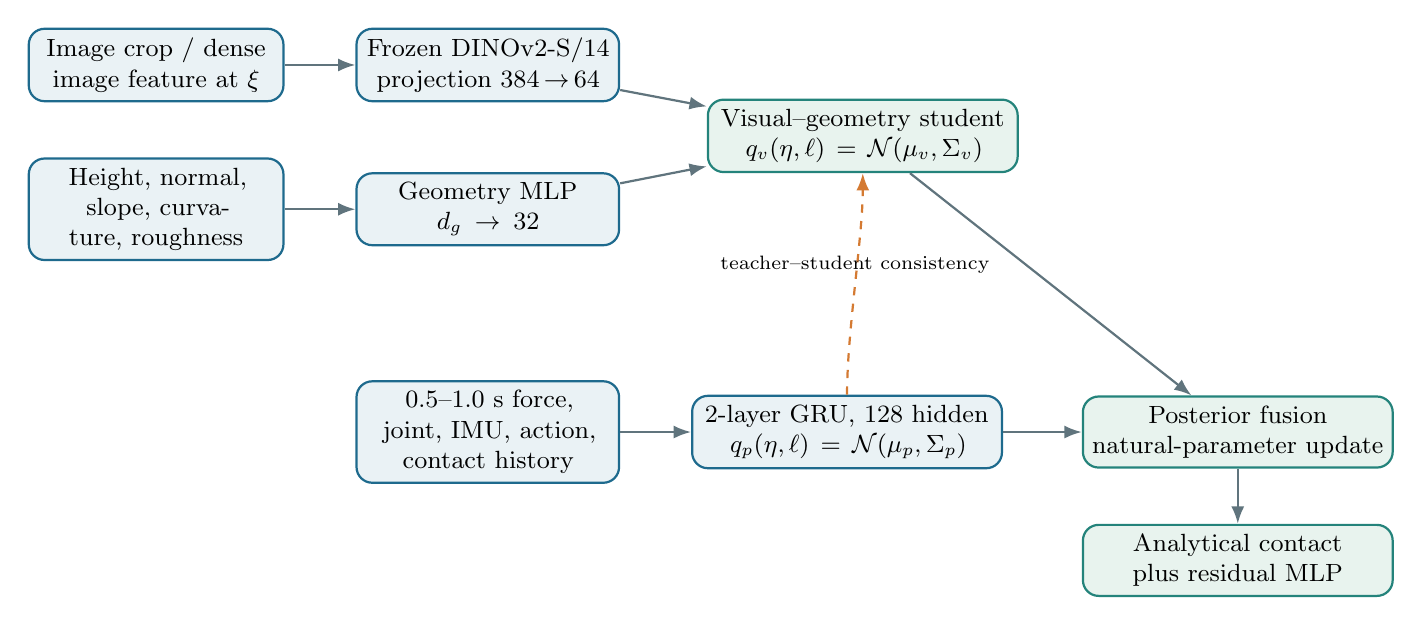
\begin{tikzpicture}[node distance=7mm and 9mm]
  \node[block,text width=30mm] (img) {Image crop / dense image feature at $\xi$};
  \node[block,right=of img,text width=31mm] (vis) {Frozen DINOv2-S/14\\projection $384\!\to\!64$};
  \node[block,below=of img,text width=30mm] (geo) {Height, normal, slope, curvature, roughness};
  \node[block,right=of geo,text width=31mm] (geomlp) {Geometry MLP\\$d_g\!\to\!32$};
  \node[physics,right=11mm of vis,text width=37mm,yshift=-9mm] (student) {Visual--geometry student\\$q_v(\eta,\ell)=\N(\mu_v,\Sigma_v)$};

  \node[block,below=17mm of geomlp,text width=31mm] (hist) {$0.5$--$1.0$ s force, joint, IMU, action, contact history};
  \node[block,right=of hist,text width=37mm] (teacher) {2-layer GRU, 128 hidden\\$q_p(\eta,\ell)=\N(\mu_p,\Sigma_p)$};
  \node[physics,right=10mm of teacher,text width=37mm] (fuse) {Posterior fusion\\natural-parameter update};
  \node[physics,below=of fuse,text width=37mm] (contact) {Analytical contact\\plus residual MLP};

  \draw[arrow] (img) -- (vis);
  \draw[arrow] (geo) -- (geomlp);
  \draw[arrow] (vis) -- (student);
  \draw[arrow] (geomlp) -- (student);
  \draw[arrow] (hist) -- (teacher);
  \draw[arrow] (student) -- (fuse);
  \draw[arrow] (teacher) -- (fuse);
  \draw[arrow] (fuse) -- (contact);
  \draw[feedback] (teacher.north) .. controls +(0,8mm) and +(0,-8mm) .. node[above,font=\scriptsize]{teacher--student consistency} (student.south);
\end{tikzpicture}
}
\caption{Cross-modal architecture. Visual prediction is a prior for untouched cells; post-contact evidence provides a teacher and online correction. The contact residual is conditioned on the fused low-dimensional posterior and instantaneous foot state.}
\label{fig:architecture}
\end{figure}

The proposed default is intentionally small:
\begin{itemize}
  \item \textbf{visual encoder:} frozen DINOv2 ViT-S/14 dense patch features \citep{oquab2023dinov2}; a two-layer projection head maps 384 dimensions to $d_z=64$;
  \item \textbf{geometry encoder:} two-layer MLP, hidden width 64, output $d_g=32$;
  \item \textbf{visual posterior head:} fused $[z,g]$ through a three-layer MLP, width 128, output mean and log variance for $\eta$ and residual latent $\ell\in\R^8$;
  \item \textbf{response teacher:} two-layer GRU with hidden size 128 over $0.5$--$1.0$ s of joint, IMU, foot-force, contact, and action history, followed by a Gaussian posterior head;
  \item \textbf{force residual:} three-layer MLP, width 128, SiLU activations, shared across feet, outputting mean and heteroscedastic log variance for $\Delta f$; and
  \item \textbf{epistemic uncertainty:} three to five independently initialized heads/ensembles, with the visual backbone shared and frozen.
\end{itemize}

This architecture is small enough for a single 16--24 GB GPU. Backbone freezing reduces overfitting to a small terrain dataset and makes online updates safe. Alternative encoders are treated as an ablation, not the central research variable.

\subsection{Cross-modal posterior fusion}

For diagonal Gaussian visual and proprioceptive posteriors, a product-of-experts update gives
\begin{align}
\Sigma_\xi^+ &= \left[(\Sigma_\xi^v)^{-1}+(\Sigma_\xi^p)^{-1}\right]^{-1},\\
\mu_\xi^+ &= \Sigma_\xi^+\left[(\Sigma_\xi^v)^{-1}\mu_\xi^v+(\Sigma_\xi^p)^{-1}\mu_\xi^p\right].
\label{eq:gaussian_fusion}
\end{align}
The teacher covariance is inflated according to force-label uncertainty and contact excitation. For example, a brief low-load normal touch should not collapse uncertainty in tangential friction. Dimensions not sufficiently excited retain their visual prior. In implementation, this is achieved with an excitation mask derived from the sensitivity matrix in \cref{eq:fisher}.

To avoid overconfident extrapolation, uncertainty contains three terms:
\begin{equation}
\Sigma_\xi^{\mathrm{total}}=
\underbrace{\E_m[\Sigma_{\xi,m}^{\mathrm{alea}}]}_{\text{sensor/contact noise}}
+\underbrace{\V_m[\mu_{\xi,m}]}_{\text{ensemble disagreement}}
+\underbrace{\Sigma_\xi^{\mathrm{map}}}_{\text{registration/age}}.
\label{eq:uncertainty_decomp}
\end{equation}
An evidential or feature-distance OOD score, inspired by PIETRA \citep{cai2024pietra}, increases the prior variance when $[z,g]$ lies far from the training manifold. It never replaces the ensemble calibration test.

\subsection{Response function and the role of visual change}

For robot state $x_t$ and action sequence $U=(u_t,\ldots,u_{t+H-1})$, the physically meaningful response function is
\begin{equation}
\hat{\mathcal R}_\Theta(z,g,x_t,U)=
\operatorname{Rollout}\left(x_t,U; q_v(\eta,\ell\mid z,g),f_\theta,\text{Eq.}\,\eqref{eq:rigid_body}\right),
\label{eq:response_function}
\end{equation}
where $\mathcal R$ contains future state, force, contact mode, slip, sinkage, tracking error, and stability quantities. The requested ``change'' relation is retained at this response level:
\begin{equation}
\Delta\hat{\mathcal R}_*=
\hat{\mathcal R}_\Theta(z_*,g_*,x_t,U)
-\hat{\mathcal R}_\Theta(z_{\mathrm{cur}},g_{\mathrm{cur}},x_t,U).
\label{eq:delta_response}
\end{equation}
Thus $\Delta z$ is never interpreted in isolation. Both counterfactuals use the same current state and action, which isolates the predicted effect of terrain. A Jacobian $J_z=\partial\hat{\mathcal R}/\partial z$ is valid only for small changes and is used for sensitivity analysis, not as the primary nonlinear model.

\subsection{Training objectives}

Training uses staged losses rather than a single end-to-end objective from the beginning.

\paragraph{Force likelihood.}
For measured contact force $f^{\mathrm{meas}}$ and predicted diagonal covariance $\Sigma_f$,
\begin{equation}
\Lcal_f=\frac{1}{2}\sum_{e,t}
\left[(f^{\mathrm{meas}}-\hat f)^\top\Sigma_f^{-1}(f^{\mathrm{meas}}-\hat f)
+\log|\Sigma_f|\right].
\label{eq:force_nll}
\end{equation}

\paragraph{Multi-step state rollout.}
Starting from measured $x_t$, the model is rolled for $K$ steps using recorded commands:
\begin{equation}
\Lcal_{\mathrm{roll}}=\sum_{k=1}^{K}\gamma_k
\left(\lVert r_{t+k}-\hat r_{t+k}\rVert_{W_r}^2+
d_R(R_{t+k},\hat R_{t+k})^2+
\lVert\nu_{t+k}-\hat\nu_{t+k}\rVert_{W_\nu}^2\right),
\label{eq:rollout_loss}
\end{equation}
where $d_R$ is geodesic orientation error. Teacher forcing is gradually reduced by scheduled sampling.

\paragraph{Visual teacher--student consistency.}
After a terrain cell has been physically excited, the visual prior is trained toward the stop-gradient response posterior:
\begin{equation}
\Lcal_{\mathrm{vis}}=
D_{\mathrm{KL}}\left(\operatorname{sg}[q_p(\eta,\ell\mid H^{p,f})]\;\Vert\;q_v(\eta,\ell\mid z,g)\right).
\label{eq:vis_distill}
\end{equation}
The reverse direction is not used, because appearance must not overwrite force evidence.

\paragraph{Physics and change consistency.}
\begin{align}
\Lcal_{\mathrm{phys}} &=
\lambda_n[-\hat f_n]_+^2+
\lambda_c[\lVert\hat f_t\rVert-\mu\hat f_n]_+^2+
\lambda_E[-W_{\mathrm{diss}}]_+^2+
\lambda_b\lVert\Delta f\rVert_2^2,\\
\Lcal_\Delta &=
\left\lVert
(\mathcal R_b^{\mathrm{real}}-\mathcal R_a^{\mathrm{real}})
-(\hat{\mathcal R}_b-\hat{\mathcal R}_a)
\right\rVert_{W_\Delta}^2,
\label{eq:physics_change_loss}
\end{align}
where paired episodes $a,b$ share similar state/action but differ in terrain. $\Lcal_\Delta$ directly trains the intended terrain-induced response change without pretending that $\Delta z$ alone is causal.

The final stage objective is
\begin{equation}
\Lcal=\lambda_f\Lcal_f+\lambda_x\Lcal_{\mathrm{roll}}+\lambda_v\Lcal_{\mathrm{vis}}
+\lambda_{\mathrm{phys}}\Lcal_{\mathrm{phys}}+\lambda_\Delta\Lcal_\Delta
+\lambda_{\mathrm{cal}}\Lcal_{\mathrm{cal}},
\label{eq:total_loss}
\end{equation}
where $\Lcal_{\mathrm{cal}}$ is a validation-set calibration penalty or post-hoc temperature scaling objective. Loss weights are first normalized by gradient magnitude and then fixed before final evaluation.

\subsection{Training curriculum}

\begin{table}[ht]
\centering
\caption{Training stages and frozen components. Progression is conditional on validation gates.}
\label{tab:training_stages}
\small
\begin{tabularx}{\textwidth}{@{}C{10mm}L{33mm}Y Y@{}}
\toprule
\textbf{Stage} & \textbf{Train} & \textbf{Freeze / supervision} & \textbf{Gate}\\
\midrule
0 & Coordinate, sensor, robot, and actuator calibration & No terrain learning; rigid reference surface & Force zero/bias stable; frame and timing errors bounded\\
1 & Analytical $\eta_r$ per controlled patch & Geometry and real force only & Identifiable parameters; no systematic force residual\\
2 & Response GRU and residual $r_\rho$ & Analytical backbone regularized; force and rollout supervision & Held-out contact improvement without energy/friction violations\\
3 & Visual--geometry prior $q_v$ & Backbone frozen; response posterior is teacher & Cross-terrain NLL and calibration better than terrain-class baseline\\
4 & Four-leg simulator composition & Contact and actuator modules initially frozen & Stable integration and improved full-body rollout\\
5 & Online posterior/memory & Backbone/contact weights frozen & Error falls after contacts without catastrophic local overconfidence\\
6 & Risk-aware planner & Dynamics frozen during evaluation & Safety improvement at matched progress\\
\bottomrule
\end{tabularx}
\end{table}

Default optimization uses AdamW, batch size 128--512 contact windows, learning rate $10^{-3}$ for heads/$10^{-4}$ for the residual, weight decay $10^{-4}$, gradient clipping at 1.0, and early stopping on held-out terrain NLL plus force NRMSE. These values are starting points; search is restricted to a small predeclared grid so that model selection does not consume the six-month schedule.

\subsection{Data splits that prevent shortcut learning}

Random frame splits would leak adjacent samples and terrain identity. Episodes are grouped before splitting, and the final benchmark contains:
\begin{enumerate}
  \item \textbf{leave-one-terrain-family-out:} all patches of a mechanical family held out;
  \item \textbf{same appearance, different physics:} visually similar patches with altered moisture, substrate, or compliance;
  \item \textbf{different appearance, same physics:} color/texture changes on a common mechanical base;
  \item \textbf{unseen operating condition:} held-out load, impact speed, slip direction, inclination, and controller command;
  \item \textbf{spatial boundary:} feet cross mixed terrain boundaries where one crop may contain multiple materials; and
  \item \textbf{temporal shift:} repeated/degrading contacts to test the recurrent terrain state.
\end{enumerate}
All normalization statistics and calibration temperatures are fit on training/validation groups only. Final test cells remain sealed until architecture and thresholds are frozen.

\section{Registered Local Digital Twin and Online Adaptation}
\label{sec:twin}

\subsection{A twin has aligned visual, geometric, and physical layers}

The local twin is
\begin{equation}
\M_t=\left\{\mathcal G_{\mathrm{render}},\ \T_{\mathrm{mesh/height}},\ 
\mathcal F_t:\xi\mapsto(z_\xi,g_\xi,\mu_\xi,\Sigma_\xi,\ell_\xi,s_{\xi},t_{\mathrm{last}})\right\}.
\label{eq:twin}
\end{equation}
The renderer and collision representation are distinct but share a calibrated world frame. This is the important lesson from recent visual--physical real-to-sim systems: a 3-D Gaussian Splatting (3DGS) reconstruction provides appearance, while a mesh, signed-distance field, or height map provides collision and contact geometry \citep{kerbl20233dgs,chen2026quadverse,han2025re3sim}. Photorealism alone cannot supply stable normals or contact penetration.

\begin{figure}[ht]
\centering
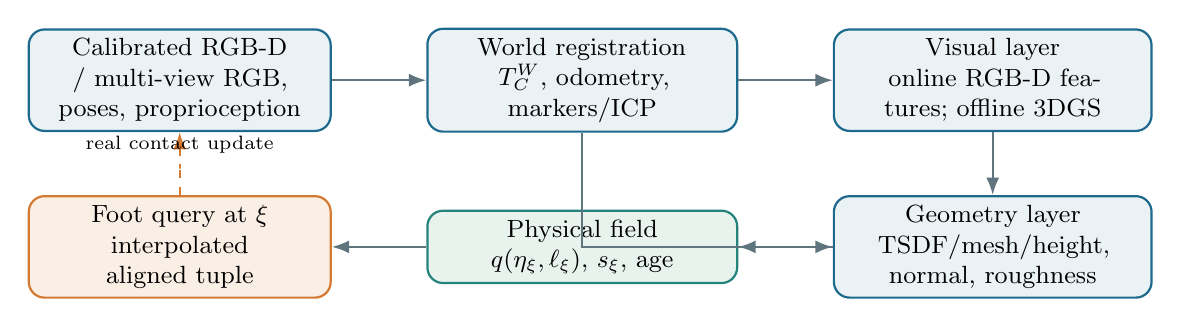
\begin{tikzpicture}[node distance=8mm and 12mm]
  \node[block,text width=36mm] (raw) {Calibrated RGB-D / multi-view RGB, poses, proprioception};
  \node[block,right=of raw,text width=37mm] (frames) {World registration\\$T_C^W$, odometry, markers/ICP};
  \node[block,right=of frames,text width=38mm] (render) {Visual layer\\online RGB-D features; offline 3DGS};
  \node[block,below=of render,text width=38mm] (geom) {Geometry layer\\TSDF/mesh/height, normal, roughness};
  \node[physics,left=of geom,text width=37mm] (phys) {Physical field\\$q(\eta_\xi,\ell_\xi)$, $s_\xi$, age};
  \node[decision,left=of phys,text width=36mm] (query) {Foot query at $\xi$\\interpolated aligned tuple};
  \draw[arrow] (raw) -- (frames);
  \draw[arrow] (frames) -- (render);
  \draw[arrow] (frames) |- (geom);
  \draw[arrow] (render) -- (geom);
  \draw[arrow] (geom) -- (phys);
  \draw[arrow] (phys) -- (query);
  \draw[feedback] (query.north) .. controls +(0,9mm) and +(0,-9mm) .. node[above,font=\scriptsize]{real contact update} (raw.south);
\end{tikzpicture}
\caption{Registered twin layers. A location is useful only when its rendered appearance, collision geometry, and physical posterior refer to the same terrain point.}
\label{fig:twin_layers}
\end{figure}

Two implementations control scope:
\begin{itemize}
  \item \textbf{fast online twin (core):} an RGB-D local height map/TSDF at 2--5 cm resolution with dense image features projected into cells. It supports contact queries and planning at runtime;
  \item \textbf{slow photorealistic twin (secondary):} an offline geometry-constrained 3DGS reconstruction from multi-view data, aligned with a collision mesh. It supports replay, camera-view augmentation, and qualitative real-to-sim evaluation, as in GaussGym/QuadVerse-style pipelines \citep{escontrela2025gaussgym,chen2026quadverse}.
\end{itemize}
The planner does not render images inside every rollout unless a visual policy is explicitly being tested. It queries cached cell features and contact posteriors; rendering is therefore not on the critical control path.

\subsection{Registration and map construction}

Camera intrinsics are calibrated once. Extrinsics $T_C^B$ are estimated with a target rigidly attached to the robot/rig, and world poses $T_B^W(t)$ come from odometry or motion capture. For a depth pixel $u$ with depth $d(u)$,
\begin{equation}
p^W=T_B^W(t)T_C^B\,d(u)K^{-1}\bar u,
\label{eq:backproject}
\end{equation}
which is fused into the geometric map. Dense visual tokens are bilinearly sampled at $u$ and accumulated in the same cell with view-angle, depth, and recency weights. The normal is estimated from local geometry; roughness and curvature use a small neighborhood but are computed at a scale no smaller than sensor noise.

Registration is validated independently of learning using known markers/edges and foot touchdown locations. The acceptance target is median terrain-point reprojection error below one map cell and touchdown-to-surface discrepancy below the foot-radius fraction relevant to the contact model. Uncertainty $\Sigma_\xi^{\mathrm{map}}$ increases with pose covariance, oblique viewing, sparse coverage, and map age.

\subsection{Online update after real contact}

When foot $i$ leaves cell $\xi$, the system packages a contact episode $e_\xi$ containing pre-contact prior, foot state/action history, measured force or inverse-dynamics force, and resulting motion. The response encoder gives $(\mu_p,\Sigma_p)$; \cref{eq:gaussian_fusion} updates the physical posterior. The residual between predicted and observed response,
\begin{equation}
e_\xi=\begin{bmatrix}f^{\mathrm{real}}-\hat f\\
\nu_{t+1:t+K}^{\mathrm{real}}-\hat\nu_{t+1:t+K}\end{bmatrix},
\label{eq:online_residual}
\end{equation}
is stored in a bounded memory. Nearby uncontacted cells receive a conservative correction through a kernel over spatial, visual, and geometric similarity:
\begin{align}
\kappa(\xi,\xi') &=
\exp\!\left[-\frac{\lVert x_\xi-x_{\xi'}\rVert^2}{2l_x^2}
-\frac{\lVert z_\xi-z_{\xi'}\rVert^2}{2l_z^2}
-\frac{\lVert g_\xi-g_{\xi'}\rVert^2}{2l_g^2}\right],\\
\Delta\mu_{\xi'} &= k_{\xi'}^\top(K+\sigma_e^2I)^{-1}e,
\label{eq:kernel_update}
\end{align}
implemented either as a sparse Gaussian process or a fixed-budget kernel dictionary. Propagation is capped, decays with distance/time, and cannot reduce variance below a calibrated floor without direct contact. This prevents a single surprising patch from rewriting an entire visually similar region.

The deployment update therefore changes only $\mu_\xi,\Sigma_\xi,\ell_\xi,s_\xi$ and the sparse memory. The DINOv2 backbone and contact network are frozen. Periodic offline retraining may incorporate accepted episodes after review, but it is not part of the real-time loop.

\begin{keybox}[Online update rule in plain language]
Before touch, trust appearance only as much as training and OOD evidence justify. After touch, let force and motion correct the contacted cell. Share that correction only with nearby cells that are similar in position, appearance, and geometry, and retain uncertainty where evidence is weak.
\end{keybox}

\section{Persistent Global Map and Topological Route Planning}
\label{sec:global}

\subsection{Why the local twin is not sufficient}

The local physical twin answers \emph{how safely can the robot execute a step or short motion on the terrain currently visible?} It does not by itself answer \emph{which side of a large concave obstacle ultimately reaches the goal?} A robot-centric local planner can be attracted toward a goal through the closed side of a U-shaped barrier, repeatedly turn away from the nearby wall, and remain trapped because leaving the U initially requires motion away from the goal.

TOP-Nav similarly maintains robot-centric goal, terrain, obstacle, and proprioception costmaps and selects a waypoint on the edge of the local map \citep{ren2024topnav}. This is effective for reactive navigation, but a persistent world-frame map and topological route search are required when the complete obstacle arrangement is larger than the local window. The added global layer is standard navigation infrastructure rather than the proposed scientific novelty; the novelty remains the visually indexed contact-response field and its physical composition.

\begin{claimbox}[Necessary distinction]
\textbf{Persistent global map and global graph search: necessary} for reliable point-goal navigation around U-shaped/cul-de-sac obstacles.\\
\textbf{Neural global time field: not necessary.} It is an optional continuous cost-to-go representation that may accelerate repeated queries or couple risk speed to an Eikonal/Hamilton--Jacobi equation after the core system works.
\end{claimbox}

\subsection{Hierarchical architecture}

\begin{figure}[ht]
\centering
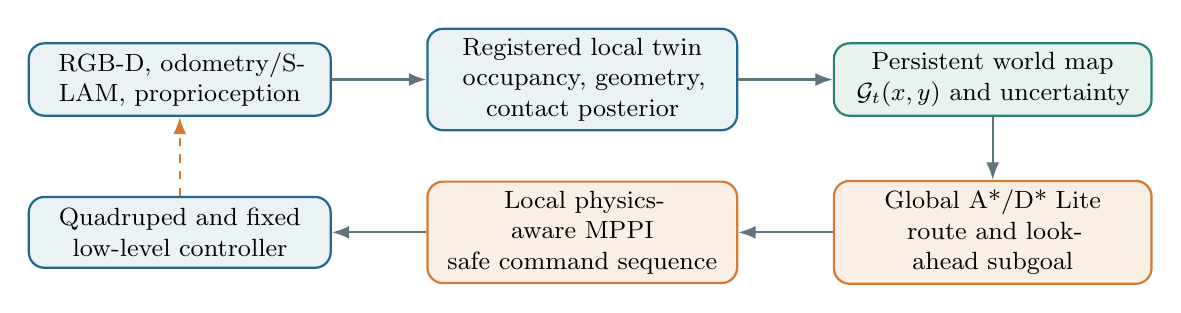
\begin{tikzpicture}[node distance=8mm and 12mm]
  \node[block,text width=36mm] (sense) {RGB-D, odometry/SLAM, proprioception};
  \node[block,right=of sense,text width=37mm] (local) {Registered local twin\\occupancy, geometry, contact posterior};
  \node[physics,right=of local,text width=38mm] (global) {Persistent world map\\$\mathcal G_t(x,y)$ and uncertainty};
  \node[decision,below=of global,text width=38mm] (route) {Global A*/D* Lite\\route and look-ahead subgoal};
  \node[decision,left=of route,text width=37mm] (mppi) {Local physics-aware MPPI\\safe command sequence};
  \node[block,left=of mppi,text width=36mm] (robot) {Quadruped and fixed low-level controller};
  \draw[arrow] (sense) -- (local);
  \draw[arrow] (local) -- (global);
  \draw[arrow] (global) -- (route);
  \draw[arrow] (route) -- (mppi);
  \draw[arrow] (mppi) -- (robot);
  \draw[feedback] (robot) -- (sense);
\end{tikzpicture}
\caption{Global--local hierarchy. The global planner resolves obstacle topology and supplies a subgoal; the local twin and MPPI determine whether and how that subgoal can be reached safely under uncertain foot--terrain physics.}
\label{fig:global_hierarchy}
\end{figure}

The global planner never commands joints. It produces a route $P_t^*$ and selects a look-ahead point $p_t^{\mathrm{sub}}$ where the route intersects the local planning horizon. MPPI then searches velocity commands that move toward $p_t^{\mathrm{sub}}$ while respecting contact, stability, and collision constraints. Thus the two questions are separated:
\begin{equation}
\underbrace{\mathcal G_t,p_{\mathrm{goal}}\longmapsto P_t^*,p_t^{\mathrm{sub}}}_{\text{where to go globally}},
\qquad
\underbrace{\M_t,x_t,p_t^{\mathrm{sub}}\longmapsto u_t}_{\text{how to move safely locally}}.
\label{eq:global_local_interface}
\end{equation}

\subsection{Persistent world-frame map}

Every local depth point and terrain cell is transformed to the common world frame using \cref{eq:backproject}. The persistent grid stores
\begin{equation}
\mathcal G_t(\xi)=\left\{
L_{\xi,t}^{\mathrm{occ}},h_\xi,n_\xi,z_\xi,
\mu_{\eta,\xi},\Sigma_{\eta,\xi},\ell_\xi,s_{\xi,t},
o_{\xi,t},t_{\mathrm{last}}
\right\},
\label{eq:global_map}
\end{equation}
where $L^{\mathrm{occ}}$ is occupancy log-odds and $o\in\{\text{observed},\text{unknown}\}$. Vertical concrete, rocks, trees, and base-height collisions belong to the occupancy layer. Ground appearance, elevation, slope, and learned contact risk belong to the traversability/physical layer. These must not be conflated: the contact model is not asked to discover that a wall is impassable.

For inverse sensor model probability $p(m_\xi\mid z_t,x_t)$, occupancy is updated by
\begin{equation}
L_{\xi,t}^{\mathrm{occ}}=L_{\xi,t-1}^{\mathrm{occ}}
+\operatorname{logit}\!\left[p(m_\xi\mid z_t,x_t)\right]-L_0,
\label{eq:occupancy_update}
\end{equation}
with clamping and pose-uncertainty inflation. Visual features use view-weighted averaging; geometry uses TSDF/height fusion; contact posteriors use \cref{eq:gaussian_fusion}. Cells remain uncertain when observation angle, localization, or physical evidence is weak. A rolling high-resolution local grid may coexist with a coarser persistent global grid of approximately 5--15 cm cells.

\subsection{Global risk cost and route search}

For a global state cell $\xi$ and heading bin $\psi$, define
\begin{align}
c_G(\xi,\psi)=&\ w_o c_{\mathrm{occ}}(\xi)
+w_r\E[R_{\mathrm{terrain}}(\xi,\psi)]
+w_\sigma\sqrt{\V[R_{\mathrm{terrain}}(\xi,\psi)]}\\
&+w_hc_{\mathrm{slope/height}}(\xi,\psi)
+w_u\mathbf 1_{\mathrm{unknown}}(\xi),
\label{eq:global_cost}
\end{align}
where $c_{\mathrm{occ}}=\infty$ for inflated occupied cells. The expected risk may initially be a conservative scalar derived from local rollouts; heading dependence is retained whenever slope direction or anisotropic slip matters. The route is
\begin{equation}
P_t^*=\arg\min_{P:\,x_t\leadsto p_{\mathrm{goal}}}
\sum_{k\in P}\left[c_G(\xi_k,\psi_k)+
\lambda_\psi d(\psi_{k+1},\psi_k)^2\right].
\label{eq:global_path}
\end{equation}

A* is the simplest known-map baseline. D* Lite is the preferred online implementation because newly observed walls or changed risk update only affected route costs rather than forcing an entirely new search. If the U is not yet fully observed, the robot treats unseen cells with a configurable uncertainty penalty, moves only toward a safe route/frontier, fuses new geometry, and replans. No planner can route around completely unseen geometry without exploration or a prior map.

\subsection{How the U-shaped concrete case is resolved}

\begin{figure}[ht]
\centering
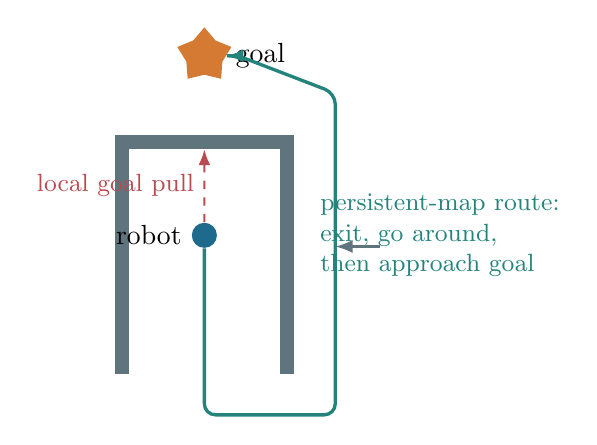
\begin{tikzpicture}[scale=0.95]
  \draw[line width=5pt,draw=muted] (0,0) -- (0,3.1) -- (2.2,3.1) -- (2.2,0);
  \node[circle,fill=blue,inner sep=3.2pt,label=left:{robot}] (r) at (1.1,1.85) {};
  \node[star,star points=5,fill=orange,draw=orange,minimum size=7mm,label=right:{goal}] (g) at (1.1,4.25) {};
  \draw[red,dashed,-{Latex[length=2mm]},thick] (r) -- node[left,font=\small]{local goal pull} (1.1,3.0);
  \draw[teal,-{Latex[length=2.2mm]},very thick,rounded corners]
    (r) -- (1.1,-0.55) -- (2.85,-0.55) -- (2.85,3.75) -- (1.55,4.25) -- (g);
  \node[align=left,font=\small,text=teal] at (4.25,1.85) {persistent-map route:\\exit, go around,\\then approach goal};
  \draw[arrow] (3.45,1.7) -- (2.85,1.7);
\end{tikzpicture}
\caption{U-shaped obstacle benchmark. A local goal attraction points into the closed wall. Persistent mapping plus A*/D* finds a temporarily goal-opposing route through the opening and around the obstacle. The local physical planner evaluates the safety of the ground along that route.}
\label{fig:u_shape}
\end{figure}

The benchmark will include mapped and incrementally revealed U-shaped/cul-de-sac layouts. Reported quantities are escape success, collision/stall rate, time to first valid detour, replanning count, path-length ratio to the known-map optimum, and physical-risk cost. The required comparison is local greedy/TOP-Nav-style edge waypoint selection versus persistent A* and D* Lite, all using the same local obstacle and terrain estimates.

\subsection{Is a global time field necessary?}

No. A global \emph{map} is necessary for topological memory; a global \emph{time field} is one possible route representation on that map. Given a risk-adjusted progress speed $S_{\mathrm{risk}}(x)$, the arrival-time field satisfies
\begin{equation}
S_{\mathrm{risk}}(x)=\max\{\epsilon,\E[v_{\mathrm{progress}}(x)]-\beta\sqrt{\V[v_{\mathrm{progress}}(x)]}\},
\qquad
\lVert\nabla T(x)\rVert=\frac{1}{S_{\mathrm{risk}}(x)}.
\label{eq:eikonal}
\end{equation}
Following $-\nabla T$ produces a continuous route to the goal, and a learned NTFields representation may answer many start--goal cost queries quickly without expert paths \citep{ni2023ntfields,liu2025active}. This is the motivation for retaining it as a stretch module. It was not required by the original contact-response idea and should not be made a dependency of its success.

\begin{table}[ht]
\centering
\caption{Role of the global planning alternatives.}
\label{tab:global_planners}
\small
\begin{tabularx}{\textwidth}{@{}L{29mm}Y Y@{}}
\toprule
\textbf{Planner} & \textbf{Why use it} & \textbf{Decision for this UGP}\\
\midrule
A* & Transparent discrete optimum on a known static grid; directly solves the U-shape topology & Required baseline\\
D* Lite & Efficient replanning when newly observed occupancy/risk changes & Core global planner\\
Fast Marching / Eikonal & Smooth continuous arrival-time field for isotropic speed/cost & Optional comparison\\
NTFields / Active NTFields & Amortized differentiable arrival-time prediction; potential repeated-query speedup & Stretch only, after map/contact validation\\
$SE(2)$ graph or anisotropic HJ & Correct when risk depends strongly on heading, gait, or slope direction & Use directional graph if needed; neural HJ is future work\\
\bottomrule
\end{tabularx}
\end{table}

An ordinary scalar 2-D time field cannot faithfully represent strongly heading-dependent quadruped risk. The safe core is therefore a directional A*/D* graph when anisotropy matters. Neural time fields are evaluated only if they improve runtime or path quality over this transparent baseline without weakening safety or interpretability.


\section{Action-Conditioned Prediction and Risk-Aware Planning}
\label{sec:planning}

\subsection{Control hierarchy and candidate actions}

The low-level locomotion controller remains fixed. The local planner searches a short sequence of high-level commands
\begin{equation}
u_t=[v_x^{\mathrm{cmd}},v_y^{\mathrm{cmd}},\omega_z^{\mathrm{cmd}}]
\label{eq:action}
\end{equation}
at 5--10 Hz over a 1.5--2.0 s horizon. Optional gait frequency or body-height offsets are added only after the three-dimensional command space is stable. For every candidate sequence, contact parameters are sampled from the map posterior and the coupled equations are rolled out. The predicted observables include progress, tracking error, base roll/pitch, support margin, slip velocity/distance, normal impulse, sinkage, foot collision, torque, and energy.

\subsection{Risk-sensitive objective}

For candidate $U$, sampled terrain/contact realization $m$, and rollout cost $J^{(m)}(U)$,
\begin{align}
J^{(m)}(U)&=\sum_{k=0}^{H-1}\Big[
w_g\lVert p_k-p_k^{\mathrm{ref}}\rVert^2
+w_v\lVert v_k-v_k^{\mathrm{cmd}}\rVert^2
+w_o\lVert\operatorname{Log}(R_k^{\mathrm{ref}\top}R_k)\rVert^2 \\
&\qquad+w_s\sum_i\lVert v_{t,i}\rVert^2\mathbf1_{c_i}
+w_\delta\sum_i\delta_i^2
+w_\tau\lVert\tau_k\rVert^2
+w_c\,\mathbf1_{\mathrm{collision}}
+w_u\operatorname{tr}(\Sigma_{R,k})\Big]+c_T,\\
J_{\mathrm{risk}}(U)&=\E_m[J^{(m)}(U)]
+\beta\,\risk_\alpha(J^{(m)}(U)).
\label{eq:risk_cost}
\end{align}
CVaR focuses the planner on the worst plausible posterior samples, a useful property for uncertain terrain \citep{rockafellar2000cvar,cai2024pietra}. Hard rejection constraints apply when predicted roll/pitch, base collision, sinkage, slip, joint limits, or solver non-convergence exceed safe thresholds.

\subsection{MPPI update}

Model Predictive Path Integral control samples perturbations around a nominal command sequence \citep{williams2018mppi}:
\begin{align}
U^{(m)}&=\bar U+\epsilon^{(m)},\qquad \epsilon^{(m)}\sim\N(0,\Sigma_U),\\
w_m&=\frac{\exp[-(J_{\mathrm{risk}}^{(m)}-J_{\min})/\lambda]}{\sum_j\exp[-(J_{\mathrm{risk}}^{(j)}-J_{\min})/\lambda]},\\
\bar U&\leftarrow \bar U+\sum_m w_m\epsilon^{(m)}.
\label{eq:mppi}
\end{align}
After two to five iterations, only the first command is executed; the horizon shifts and replans with new measurements. A realistic starting budget is 512--2048 candidate rollouts, 8--16 posterior samples shared through common random numbers, and vectorized integration. If full contact rollouts miss the runtime budget, a GRU surrogate is distilled from the validated simulator for planning speed, but its predictions are screened against the physical model on a smaller elite set.

\subsection{Runtime and safety fallback}

The target timing hierarchy is:
\begin{table}[ht]
\centering
\caption{Runtime targets and degradation strategy.}
\label{tab:runtime}
\begin{tabularx}{\textwidth}{@{}L{35mm}L{30mm}Y@{}}
\toprule
\textbf{Module} & \textbf{Target} & \textbf{If the budget is missed}\\
\midrule
Low-level controller & 200--500 Hz & Never slowed by perception/planning\\
Contact/dynamics integration & 200--500 Hz internal step & Fewer candidate actions; cached features; compiled/batched model\\
Local map update & 10--20 Hz & Coarser cells and asynchronous feature projection\\
Persistent map / D* update & 1--5 Hz or event-driven & Coarser global grid; incremental affected-cell replanning\\
MPPI replanning & 5--10 Hz & Shorter horizon, fewer samples, distilled surrogate plus elite recheck\\
Photorealistic reconstruction & offline & No impact on control loop\\
\bottomrule
\end{tabularx}
\end{table}

When all candidate trajectories violate constraints or OOD uncertainty exceeds a threshold, the robot does not extrapolate aggressively. It switches to a conservative command envelope: reduce speed, shorten step, stop before the uncertain patch, or request a low-load exploratory touch if the controller supports it. Emergency stops and joint/tilt limits remain outside the learned system.

\section{Experimental Evaluation}
\label{sec:evaluation}

\subsection{Evaluation ladder}

The validation order mirrors the causal structure of the method. A later claim is made only if the earlier interface has passed.

\begin{enumerate}
  \item \textbf{Sensor and rigid-floor calibration:} timing, frame transforms, actuator residual, force noise, and repeatability.
  \item \textbf{Single-contact interpolation:} held-out loads/speeds on known terrain patches.
  \item \textbf{Single-contact extrapolation:} held-out terrain family and appearance/physics ambiguity tests.
  \item \textbf{Four-leg composition in simulation:} same local law under changing multi-foot load distribution, gait, and commands.
  \item \textbf{Limited whole-robot validation:} safe, low-speed traversal over controlled patches if hardware is available.
  \item \textbf{Online adaptation:} error and calibration before/after one to five contacts.
  \item \textbf{Global topology:} mapped and incrementally revealed U-shaped/cul-de-sac layouts, comparing local-only waypoints with persistent A*/D* routes.
  \item \textbf{Closed-loop physical planning:} repeated navigation trials at matched progress and command limits.
\end{enumerate}

This ladder avoids using planning success to hide an inaccurate physical model. Contact, composition, perception, uncertainty, and planning are reported separately before an end-to-end result.

\subsection{Metrics}

\begin{table}[ht]
\centering
\caption{Metrics reported by subsystem.}
\label{tab:metrics}
\small
\begin{tabularx}{\textwidth}{@{}L{27mm}Y Y@{}}
\toprule
\textbf{Subsystem} & \textbf{Primary metrics} & \textbf{Diagnostic metrics}\\
\midrule
Contact force & Axis-wise RMSE/NRMSE; normal impulse error; tangential direction error; slip-onset F1; sinkage MAE & Friction-cone violation; passive-energy violation; error versus load/speed/angle; spectral error\\
Coupled rollout & Base position/velocity MAE; roll/pitch geodesic error; joint-state error; contact timing F1; 0.25/0.5/1.0 s drift & Per-foot force distribution; solver failures; error accumulation slope\\
Visual prior & NLL; posterior coverage at 50/80/90/95\%; expected calibration error; OOD AUROC & Same-appearance/different-physics confusion; parameter/latent sensitivity\\
Online update & Error after 0,1,2,5 contacts; uncertainty contraction; negative transfer rate & Memory size, update latency, spatial decay, forgetting\\
Global mapping/route & U-shape escape success; collision/stall; path ratio to known-map optimum; replanning latency & Occupancy IoU; localization drift; unknown-cell exposure; number of route reversals/replans\\
Planning & Success; fall/stall; slip distance/events; worst-case/CVaR cost; completion time; energy per meter & Clearance, tilt, intervention rate, computation time and missed deadlines\\
Twin registration & Reprojection error; foot touchdown-to-surface error & Map age, pose covariance, feature consistency across views\\
\bottomrule
\end{tabularx}
\end{table}

Normalized force error is
\begin{equation}
\operatorname{NRMSE}(f_j)=
\frac{\sqrt{\frac{1}{N}\sum_t(f_{j,t}-\hat f_{j,t})^2}}
{f_{j,95\%}^{\mathrm{meas}}-f_{j,5\%}^{\mathrm{meas}}+\epsilon},
\label{eq:nrmse}
\end{equation}
which is less distorted by impact outliers than normalization by the absolute maximum. Uncertainty is accepted only if coverage is close to nominal and interval width is useful; a trivially wide interval does not count as calibrated performance.

\subsection{Baselines}

\begin{table}[ht]
\centering
\caption{Baselines isolate where performance comes from.}
\label{tab:baselines}
\small
\begin{tabularx}{\textwidth}{@{}C{8mm}L{38mm}Y@{}}
\toprule
\textbf{ID} & \textbf{Baseline} & \textbf{Question answered}\\
\midrule
B0 & Uniform rigid/contact simulator & Does any terrain adaptation help?\\
B1 & Per-terrain oracle fitted parameters & Upper bound for known patches; separates visual error from contact-model error\\
B2 & Visual terrain class to fixed friction & Is a semantic/scalar model sufficient?\\
B3 & Vision-to-friction/stiffness point estimate \citep{chen2024terrain} & Does posterior/residual/history add value?\\
B4 & Black-box perceptive forward dynamics \citep{roth2025perceptive} & Does explicit contact composition improve transfer, diagnosis, or data efficiency?\\
B5 & Hybrid contact law without visual prior & What is gained before first contact?\\
B6 & Hybrid contact law without online update & What is gained from reality feedback?\\
B7 & Full model, deterministic mean only & Does uncertainty-aware planning help?\\
B8 & Full model with oracle map labels & How much error is caused by registration/perception rather than dynamics?\\
B9 & Robot-centric local edge-waypoint planner & Does persistent world-frame memory remove U-shape/cul-de-sac local minima?\\
B10 & Persistent A* versus D* Lite versus time field & Is incremental or neural/global-field complexity justified by path quality or replanning time?\\
\bottomrule
\end{tabularx}
\end{table}

All baselines receive the same state estimator, low-level controller, geometry map, command bounds, training episodes where applicable, and planner sample budget. The oracle is not presented as deployable.

\subsection{Ablations}

The following ablations are predeclared:
\begin{itemize}
  \item analytical law only versus analytical plus residual;
  \item memoryless versus recurrent terrain state;
  \item no geometry, no visual feature, and no contact history;
  \item friction-only versus friction plus compliance/damping;
  \item visual student trained on class/parameter labels versus response-posterior distillation;
  \item independent per-foot rollout versus fully coupled equation \eqref{eq:rigid_body};
  \item uncalibrated versus calibrated/frozen actuator residual;
  \item point estimate versus aleatoric uncertainty versus ensemble total uncertainty;
  \item direct-cell update versus spatial/feature kernel propagation;
  \item coarse terrain regions versus fine-grained contact field; and
  \item physics rollouts versus distilled fast forward surrogate for planning;
  \item robot-centric local map versus persistent world-frame map; and
  \item A* versus D* Lite versus Fast Marching/time field on identical global costs.
\end{itemize}

\subsection{Concrete acceptance criteria and decision gates}

The numbers below are targets suitable for mentor review, not fabricated expected results. They create honest stop/go decisions.

\begin{table}[ht]
\centering
\caption{Proposed success and fallback gates.}
\label{tab:gates}
\small
\begin{tabularx}{\textwidth}{@{}L{24mm}Y Y@{}}
\toprule
\textbf{Gate} & \textbf{Proceed criterion} & \textbf{Fallback if missed}\\
\midrule
G0: measurement & Force bias $<2\%$ of test range; timing error $<2$ high-rate samples; rigid-floor repeatability documented & Recalibrate; reduce claims to simulation/inverse-dynamics study\\
G1: local law & Held-out normal-force NRMSE $\le15\%$, tangential $\le25\%$, impulse error $\le15\%$, and $\ge20\%$ relative improvement over B0 & Simplify $\eta$, improve excitation, restrict supported operating envelope\\
G2: physical validity & $<1\%$ friction/passivity violations after hard projection; stable integration over test episodes & Reduce residual magnitude, step size, or contact stiffness; use implicit solve\\
G3: composition & At 0.5 s, base velocity MAE $\le 0.15$ m/s and roll/pitch MAE $\le3^\circ$, with improvement over B0/B4 & Report simulation composition only; collect targeted multi-contact calibration\\
G4: perception & Full model beats B2/B3 in leave-one-family-out NLL; 90\% coverage lies in 85--95\% band & Retain high uncertainty; treat vision only as a broad prior\\
G5: adaptation & Median force/response error drops after $\le5$ contacts without increasing OOD overconfidence & Use direct-cell updates only; remove kernel propagation\\
G6: global topology & At least 95\% mapped-U escape success and 90\% incrementally revealed-U success, with median path length $\le1.35\times$ known-map optimum & Retain A* on complete maps; restrict unknown-space claim; diagnose SLAM versus planning failure\\
G7: local planning & $\ge25\%$ reduction in slip/fall/stall events versus deterministic B7 at matched progress, with no more than 20\% runtime penalty & Demonstrate prediction/global-route system; leave physics-aware closed-loop planning as future work\\
\bottomrule
\end{tabularx}
\end{table}

The exact G0 threshold will be adjusted to the actual sensor specification before data collection. G1--G7 remain frozen once a pilot set establishes feasible normalization and safety bounds.

\subsection{Statistical protocol}

Every final navigation condition uses at least 20 repeated trials per method if simulation-only and at least 8--10 safe repeats per method on hardware, subject to material reset and safety constraints. The global benchmark additionally samples at least 50 U/cul-de-sac geometries with varied opening direction, wall length, partial observability, terrain cost, and localization noise. Method order is randomized; terrain preparation, moisture/compaction, battery state, and ambient light are logged. Continuous metrics use paired bootstrap 95\% confidence intervals over episode differences. Binary success uses Wilson intervals and Fisher's exact/permutation tests. Effect sizes and confidence intervals are reported alongside $p$-values. Multiple primary comparisons use Holm correction. Seeds, failed runs, solver failures, and interventions are included rather than silently discarded.

\subsection{Whole-robot validation under limited access}

The real quadruped validation set is intentionally small and safe:
\begin{enumerate}
  \item slow stance load shifts on two adjacent controlled surfaces;
  \item low-speed straight traversal across a rigid-to-compliant or high-to-low-friction boundary;
  \item a held-out patch with a conservative stop/fallback policy; and
  \item repeated contact at one deformable cell to test $s_\xi$; and
  \item if space permits, low-speed navigation through a lightweight U-shaped barrier while the global route is logged.
\end{enumerate}
Motion capture or accurate visual-inertial odometry, joint/IMU logs, and video are collected; foot force sensing is used if available. Without real full-body data, the report will state: ``real single-leg contact validation plus four-leg simulation composition.'' It will not claim a fully validated real quadruped digital twin.

\subsection{Reproducibility package}

The final package will contain sensor calibration, synchronized data schema, train/validation/test episode lists, terrain preparation sheets, configuration files, random seeds, contact plug-in interface, model checkpoints, local/global mapping calibration, U-shape world definitions, simulator version, evaluation scripts, and a one-command representative benchmark. Raw personally identifying imagery is excluded or blurred; laboratory safety and equipment-use rules take precedence over data collection volume.

\section{Six-Month Execution Plan}
\label{sec:execution}

\subsection{Scope tiers}

The project is structured so that a defensible result exists even if a stretch component fails.

\begin{table}[ht]
\centering
\caption{Core, target, and stretch scope.}
\label{tab:scope}
\begin{tabularx}{\textwidth}{@{}L{25mm}Y Y@{}}
\toprule
\textbf{Tier} & \textbf{Included} & \textbf{Result if completed}\\
\midrule
Core & Calibrated single-leg dataset; analytical plus residual 3-D contact law; four-leg simulator plug-in; persistent occupancy/elevation map and A*/D* route baseline & A strong physics/learning UGP with a publishable composition question and complete navigation infrastructure\\
\addlinespace[2pt]
Target & Registered RGB-D physical field; visual prior; limited online correction; physics-aware MPPI; safe quadruped trials if available & Full hierarchical visuo-proprioceptive digital twin claim\\
\addlinespace[2pt]
Stretch & Offline 3DGS rendering; deformable mud state; MPPI on hardware; Fast Marching/anisotropic HJ/NTFields comparison & Expanded real-to-sim and neural-field navigation study\\
\bottomrule
\end{tabularx}
\end{table}

The ordering is non-negotiable: \textbf{single-leg law $\rightarrow$ four-leg coupling $\rightarrow$ registered local twin $\rightarrow$ persistent global map/D* route $\rightarrow$ online adaptation and local MPPI}. A visually impressive twin or neural time field is not built before the contact interface and transparent global baseline are trustworthy.

\subsection{Week-by-week plan and milestones}

\begin{longtable}{@{}C{16mm}L{39mm}p{88mm}@{}}
\caption{Detailed 26-week execution plan.}\label{tab:schedule}\\
\toprule
\textbf{Weeks} & \textbf{Milestone} & \textbf{Work and exit artifact}\\
\midrule
\endfirsthead
\toprule
\textbf{Weeks} & \textbf{Milestone} & \textbf{Work and exit artifact}\\
\midrule
\endhead
1--2 & M0: specification & Freeze coordinate frames, signals, terrain tiers, supported load/speed envelope, safety limits, and evaluation splits. Deliver interface/control document.\\
3 & M1: calibration & Calibrate camera, rig kinematics, force bias/scale, time synchronization, rigid reference floor, and actuator delay/residual. Pass G0.\\
4--5 & Pilot data & Run indentation, rate, and tangential pilot. Estimate noise, check force-frame transformation, select D-optimal conditions, and freeze data schema.\\
6--7 & M2: contact dataset & Collect core surfaces with repetitions; quality-control plots after each session; seal group-wise train/validation/test lists.\\
8--9 & Analytical ID & Fit $\mu,k,c,\gamma$; compute sensitivity/Fisher spectra; reduce unidentifiable dimensions; implement force-cone projection and passivity diagnostics.\\
10 & M3: analytical baseline & Held-out report for B0/B1 and failure cases. Decide whether deformable state is justified.\\
11--12 & Residual and teacher & Train force residual and response GRU; tune only on training/validation; evaluate force, impulse, and short rollouts.\\
13 & M4: local law gate & Freeze v1 contact law after G1/G2. If missed, restrict operating envelope before continuing.\\
14--15 & Visual prior & Project frozen DINOv2 features, train geometry encoder and teacher--student posterior, calibrate ensemble, run ambiguity/OOD splits.\\
16 & M5: perception gate & Complete B2/B3 comparisons and calibration plots; pass G4 or retain vision as broad prior.\\
17--18 & Four-leg coupling & Integrate four shared contact queries with MuJoCo/robot model; implicit stepping, solver monitoring, and actuator model; run load-shift/gait tests.\\
19 & M6: composition gate & Compare B0/B4 and ablations; pass G3 for supported horizon. Prepare limited hardware protocol.\\
20 & Local/global mapping & Build RGB-D height/TSDF local map, registered physical cells, world-frame occupancy/elevation fusion, map uncertainty, and foot query API.\\
21 & Global route gate & Integrate A*/D* Lite, route-to-subgoal interface, and mapped/incremental U-shape benchmark. Attempt offline 3DGS only if the core schedule is intact.\\
22 & Online update & Implement Gaussian fusion and bounded sparse kernel memory; test direct-cell update and negative-transfer controls.\\
23 & M7: adaptation gate & Error-versus-contact curves, memory ablations, update runtime; pass G5.\\
24 & Local planner integration & MPPI follows D* subgoals using posterior sampling, CVaR cost, hard constraints, and conservative fallback; benchmark runtime.\\
25 & M8: closed-loop tests & Simulation and limited safe hardware trials; U-shape and terrain-risk baselines, randomized repeats, failure analysis; pass/report G6--G7.\\
26 & Finalization & Freeze repository/data manifest, compute confidence intervals, make figures/video, write final report and mentor handoff.\\
\bottomrule
\end{longtable}

\subsection{Resource and data budget}

\begin{table}[ht]
\centering
\caption{Expected resources.}
\label{tab:resources}
\begin{tabularx}{\textwidth}{@{}L{31mm}Y Y@{}}
\toprule
\textbf{Resource} & \textbf{Minimum} & \textbf{Preferred / use}\\
\midrule
Robot setup & Existing single-leg rig/simulator; encoder/current/torque logs & Six-axis foot F/T or force plate; limited quadruped access\\
Terrain & Four small repeatable patches & Incline fixture, moisture/compaction measurement, optional mud/organic test\\
Vision & Calibrated RGB camera & RGB-D or depth camera; multi-view capture for 3DGS\\
Compute & One modern GPU with 16 GB VRAM; 16 CPU cores & 24 GB GPU or batched simulator node\\
Storage & 300 GB for synchronized logs and models & 0.5--1 TB if retaining raw multi-view/3DGS data\\
Software & ROS/ROS2, Python, PyTorch, MuJoCo, OpenCV/Open3D & Isaac Lab for batched rollouts; COLMAP/3DGS implementation\\
People/time & One student plus weekly mentor checkpoint & Lab support for sensor mounting and safe robot trials\\
\bottomrule
\end{tabularx}
\end{table}

The project does not require repeated uncontrolled full-quadruped mud trials. Most data come from the one-leg setup and small resettable patches; whole-robot trials are validation, not the main training source.

\subsection{Risk register}

\begin{longtable}{@{}L{31mm}C{14mm}C{14mm}L{74mm}@{}}
\caption{Technical risks and planned controls.}\label{tab:risks}\\
\toprule
\textbf{Risk} & \shortstack{\textbf{Like-}\\\textbf{lihood}} & \textbf{Impact} & \textbf{Mitigation and trigger}\\
\midrule
\endfirsthead
\toprule
\textbf{Risk} & \shortstack{\textbf{Like-}\\\textbf{lihood}} & \textbf{Impact} & \textbf{Mitigation and trigger}\\
\midrule
\endhead
No reliable foot force label & Medium & High & Prefer force plate/F/T sensor. Validate inverse dynamics on rigid trials; if tangential force is unreliable, narrow claims to normal response/impulse.\\
Contact parameters unidentifiable & Medium & High & Inspect Fisher spectrum; add rate/load/direction excitation; reduce $\eta$ rather than fitting unstable constants.\\
Single-leg law does not transfer & Medium & High & Cover expected load/impact envelope; separate actuator calibration; evaluate composition before visual twin; collect a small targeted multi-contact correction set.\\
Stiff learned contact destabilizes integration & Medium & High & Positive bounded parameters, friction projection, residual regularization, semi-implicit solve, adaptive step and non-convergence flag.\\
Visual shortcut/terrain memorization & High & Medium & Grouped splits, appearance--physics counterexamples, frozen backbone, geometry ablation, OOD calibration.\\
Registration error appears as physics error & Medium & High & Independent marker/touchdown benchmark; propagate map covariance; no model training until registration gate is met.\\
Local planner becomes trapped in concave obstacles & Medium & High & Persistent world-frame occupancy map, D* Lite route, U-shape benchmark, and explicit unknown-space policy.\\
Mud/granular trials are not repeatable & High & Medium & Begin with rigid/compliant/controlled granular surfaces; log preparation; treat natural terrain as external validation.\\
Online update causes negative transfer & Medium & High & Fixed-budget local memory, variance floor, capped spatial propagation, direct-cell fallback, rollback of last update.\\
Planner misses real-time budget & Medium & Medium & Cached cell features, low-dimensional actions, vectorized rollouts, shorter horizon, distilled surrogate with elite physical recheck.\\
Insufficient quadruped access & Medium & Medium & Predeclare two claim levels; deliver real single-leg plus four-leg simulation study if hardware validation is unavailable.\\
Safety event & Low & High & Tether/gantry where appropriate, speed/tilt/torque limits, protected test zone, independent E-stop, supervised trials, conservative fallback.\\
\bottomrule
\end{longtable}

\subsection{Weekly mentor decision dashboard}

Each weekly meeting reports one page with: (i) milestone status, (ii) one primary quantitative plot, (iii) failed conditions and cause, (iv) data volume/quality, (v) next week's acceptance test, and (vi) decisions required from the mentor. This prevents the project from drifting toward photorealistic demos before the contact claim is proven.

\subsection{Final deliverables}

\begin{enumerate}
  \item calibrated synchronized single-leg terrain-interaction dataset and preparation protocol;
  \item analytical and residual contact model with uncertainty and recurrent state;
  \item four-leg dynamics integration plug-in and validation benchmark;
  \item registered visual--geometry--physical local map, with optional 3DGS reconstruction;
  \item persistent global occupancy/elevation/physical map with A*/D* route and U-shape benchmark;
  \item visual prior, response teacher, and bounded online update module;
  \item uncertainty-aware MPPI demonstration following global subgoals, with baseline/ablation suite;
  \item reproducible code, configurations, checkpoints, videos, and final report; and
  \item a concise statement of passed/failed hypotheses and the exact supported operating envelope.
\end{enumerate}

\section{Expected Scientific Outcome and Decision Case}
\label{sec:decision}

The proposal is ambitious in integration but conservative in scientific sequencing. It reuses mature components where novelty is unnecessary: a frozen visual foundation encoder, standard multibody equations, an existing low-level locomotion controller, and MPPI. Research effort is concentrated at the unresolved interface: learning a real, state-dependent, uncertain contact response from controlled interaction and proving that it composes.

The project remains successful at several levels. At minimum it can produce a careful single-leg contact benchmark, compositional simulator study, and transparent global map/D* navigation baseline. With the target modules, it becomes a pre-contact visual physical prior corrected by real response and followed by local risk-aware control. Neural time fields remain an optional representation comparison. Every level has explicit baselines and stop criteria, so negative results remain interpretable.

\begin{claimbox}[Recommended UGP formulation]
\textbf{Title:} Online Visuo-Proprioceptive Contact-Response Fields for Physically Coupled Quadruped Digital Twins.\\[1mm]
\textbf{Core claim to approve:} A local foot--terrain interaction law learned from controlled real trials can be visually indexed, uncertainty-calibrated, and composed through four-contact rigid-body dynamics to improve prediction of action-conditioned quadruped response.\\[1mm]
\textbf{Core deliverable at six months:} a validated single-leg contact model, four-leg coupled simulator, registered local physical field, persistent global map/D* route layer, and rigorous comparison against local-only, uniform, visual-parameter, and black-box forward-dynamics baselines.\\[1mm]
\textbf{Stretch deliverable:} online correction, physics-aware closed-loop hardware navigation, photorealistic reconstruction, and neural time-field comparison.
\end{claimbox}

This formulation is sufficiently focused for a six-month undergraduate project, technically deep enough to support a research contribution, and modular enough to survive hardware or reconstruction delays without losing its central scientific question.


\appendix
\section{Implementation Specification}
\label{app:implementation}

\subsection{End-to-end training procedure}

\begin{tcolorbox}[colback=paper,colframe=blue,title={Algorithm 1: staged model construction},fonttitle=\bfseries\color{navy}]
\begin{enumerate}[leftmargin=1.8em]
  \item Calibrate $K,T_C^B$, robot inertial/kinematic parameters, force transforms, clocks, and rigid-floor actuator residual $\Delta\tau_\omega$.
  \item For each terrain patch, collect synchronized episodes under the excitation design; reject only predeclared sensor faults and retain physical failures.
  \item Fit analytical $\eta_r$ with \cref{eq:sysid}; inspect \cref{eq:fisher}; reduce/fix parameters if unidentifiable.
  \item Train response teacher and residual contact model on force NLL and short rollout loss while enforcing \cref{eq:force_projection}.
  \item Extract frozen dense visual features and registered geometry for every contact point. Train $q_v$ toward stop-gradient $q_p$ using \cref{eq:vis_distill}; calibrate ensemble variance on validation groups.
  \item Freeze actuator and contact modules; plug four copies into \cref{eq:rigid_body}; test numerical stability and composition. Fine-tune only if errors are attributable and regularized.
  \item Build the registered local map, fuse it into persistent $\mathcal G_t$, and initialize observed ground cells with $q_v$. Validate A*/D* on mapped and incrementally revealed U-shaped layouts.
  \item Replay held-out contact trajectories without online updates; then enable direct-cell and sparse-memory corrections.
  \item Freeze all learning for final planning evaluation. Run D* subgoal selection and MPPI with matched map, compute, and action constraints for all baselines.
\end{enumerate}
\end{tcolorbox}

\subsection{Online deployment procedure}

\begin{tcolorbox}[colback=paper,colframe=teal,title={Algorithm 2: one receding-horizon cycle},fonttitle=\bfseries\color{navy}]
\begin{enumerate}[leftmargin=1.8em]
  \item Acquire time-aligned image/depth, $q,\nu$, IMU, and prior action; update localization covariance.
  \item Fuse depth into the local geometry map; project frozen image tokens into visible cells; update $(z_\xi,g_\xi,\Sigma_\xi^{\mathrm{map}})$.
  \item For newly visible cells, initialize $q_v(\eta_\xi,\ell_\xi)$ and OOD-inflated uncertainty.
  \item Transform observed cells to the world frame, update persistent occupancy/physical map $\mathcal G_t$, and trigger D* Lite if affected route costs changed.
  \item Select look-ahead subgoal $p_t^{\mathrm{sub}}$ on the global route. If no safe route exists, stop or choose a bounded exploration frontier rather than moving greedily toward the goal.
  \item Sample command perturbations toward $p_t^{\mathrm{sub}}$ and common-random-number contact parameters. For every candidate, repeatedly query four feet, solve \cref{eq:implicit}, update $s_\xi$, and accumulate \cref{eq:risk_cost}.
  \item Reject unsafe/non-converged candidates; update the nominal MPPI sequence with \cref{eq:mppi}. If none remain, execute conservative fallback.
  \item Execute only the first command. The independent low-level controller enforces joint-level safety.
  \item At contact completion, encode force/proprio history, fuse the contacted-cell posterior with \cref{eq:gaussian_fusion}, and update the bounded residual dictionary. Log prior, posterior, prediction, observation, and update magnitude.
\end{enumerate}
\end{tcolorbox}

\subsection{Tensor and module specification}

\begin{table}[ht]
\centering
\caption{Reference tensor dimensions. Dimensions may change with the available robot signals, but the interfaces remain fixed.}
\label{tab:tensors}
\small
\begin{tabularx}{\textwidth}{@{}L{31mm}C{25mm}Y@{}}
\toprule
\textbf{Quantity} & \textbf{Dimension} & \textbf{Contents}\\
\midrule
Dense visual token $z_\xi$ & 64 & Projected DINOv2 feature, view-fused per map cell\\
Geometry $g_\xi$ & 8--12 & Height, normal (3), slope, two curvatures, roughness, confidence\\
Effective parameter $\eta_\xi$ & 4--6 & $\mu,k,c,\gamma$; optional anisotropy ratio/direction\\
Residual latent $\ell_\xi$ & 8 & Non-interpretable local code, Gaussian posterior\\
Terrain state $s_\xi$ & 0, 2, or 4 & None for rigid; compaction/sinkage and shear/history for deformable\\
Instant foot state $\chi_i$ & 24--40 & Pose representation, linear/angular velocity, penetration/rate, load estimate, command, contact flags\\
Response history step & robot-dependent & Joint position/velocity/torque, IMU, force, action, contact flags\\
Response GRU state & 128 & Two-layer causal GRU\\
Force output & 6 & Mean and log variance for $f_x,f_y,f_z$ before hard constraint\\
Planner action & 3 core & $v_x^{cmd},v_y^{cmd},\omega_z^{cmd}$\\
Risk vector & 8--16 & Slip, tilt, sinkage, collision, tracking, torque, energy, solver health\\
Persistent map cell $\mathcal G_t(\xi)$ & 20--100 & Occupancy log-odds, observed flag, geometry, feature summary, contact posterior, uncertainty, age\\
Global route/subgoal & variable / 3 & World-frame route cells plus current $(x,y,\psi)$ look-ahead target\\
\bottomrule
\end{tabularx}
\end{table}

\subsection{Per-step simulator pseudocode}

\begin{verbatim}
inputs: q_t, nu_t, command u_t, local map M_t, terrain states s_t
tau_t = low_level_controller(q_t, nu_t, u_t) + actuator_residual(history)

initialize q_next, nu_next from previous step
repeat until converged or max_iter:
    for foot i in {1,2,3,4}:
        pose_i, vel_i, J_i = forward_kinematics(q_next, nu_next)
        xi_i, geometry_i = collide_and_query(pose_i, M_t)
        contact_sample_i = sample_or_mean(M_t.posterior[xi_i])
        f_i, cov_i = contact_model(pose_i, vel_i, u_t,
                                   geometry_i, contact_sample_i,
                                   s_t[xi_i])
    nu_new = implicit_body_solve(q_t, nu_t, tau_t, {J_i, f_i})
    q_new  = integrate_configuration(q_t, nu_new)
    damp/update q_next, nu_next

if not converged: mark rollout unsafe and reduce step/fallback
update contacted terrain states s_{t+1}
return q_next, nu_next, forces, force covariance, solver flag
\end{verbatim}

\subsection{Dataset record and quality control}

Each episode is immutable after collection and contains:
\begin{itemize}
  \item identifiers: episode, terrain patch, preparation batch, robot/foot, operator, date/time;
  \item calibration hashes: intrinsics/extrinsics, force transform, robot model, synchronization version;
  \item environment: material, depth/thickness, slope, moisture/compaction if measurable, light, temperature;
  \item commands: reference joint/foot trajectory, controller gains, high-level command, abort reason;
  \item high-rate signals: timestamps, joint states, current/torque, IMU, force/torque, estimated foot pose/velocity, contact state;
  \item image/depth frames with exposure and camera pose;
  \item derived but reproducible values: penetration, normal/tangent frames, filtered acceleration, episode quality flags; and
  \item split label assigned at the episode/patch level before model training.
\end{itemize}

Automatic QC plots show clock offsets, missing samples, force saturation, pre-contact bias, force/penetration hysteresis, commanded versus achieved motion, and camera/foot projection. A raw episode is never overwritten by filtered data.

\section{Experimental Matrix}
\label{app:matrix}

\begin{table}[ht]
\centering
\caption{Core excitation levels before D-optimal subsampling.}
\label{tab:matrix}
\small
\begin{tabularx}{\textwidth}{@{}L{34mm}Y Y@{}}
\toprule
\textbf{Factor} & \textbf{Candidate levels} & \textbf{Why it matters}\\
\midrule
Normal load / target indentation & low, nominal, high; within rig and quadruped safety envelope & Friction scales with load; compliance can be nonlinear\\
Vertical speed & quasi-static, nominal landing, high safe impact & Separates stiffness, damping, and impulse behavior\\
Tangential speed & zero, pre-slip, sliding; forward/lateral/diagonal & Friction transition, directionality, residual shear\\
Foot orientation & level plus positive/negative pitch and roll & Edge/area contact and frame sensitivity\\
Terrain inclination & level, moderate uphill/downhill/cross-slope & Geometry--physics interaction and anisotropy\\
Contact repetition & fresh, 2nd, 5th, 10th contact & Compaction, hysteresis, recovery\\
Appearance condition & normal light, shadow, changed color/cover & Tests visual robustness without changing physics\\
Material condition & matched appearance with altered backing/moisture where reproducible & Exposes failure of semantic shortcuts\\
\bottomrule
\end{tabularx}
\end{table}

For four core surfaces, 100--150 short selected episodes per surface give 400--600 training/validation episodes plus 80--120 sealed test episodes. Impact and boundary trials are collected separately. Actual count is determined by force variability: collection stops only when bootstrap confidence on repeatability is adequate, not at an arbitrary image count.

\section{Failure Taxonomy and Interpretation}
\label{app:failures}

\begin{table}[ht]
\centering
\caption{How failures will be diagnosed rather than collapsed into ``model error.''}
\label{tab:failure_taxonomy}
\small
\begin{tabularx}{\textwidth}{@{}L{31mm}Y Y@{}}
\toprule
\textbf{Observed failure} & \textbf{Likely discriminator} & \textbf{Action}\\
\midrule
Force error on rig, all terrains & Frame/timing/force calibration, actuator/fixture dynamics & Stop learning; repair G0\\
Good force, poor one-step body acceleration & Robot inertial/Jacobian model or force application point & Recalibrate mechanics/contact point\\
Good one-step, diverging multi-step rollout & Contact stiffness/integration, controller delay, state-estimation bias & Implicit solve, smaller step, actuator residual\\
Known terrain good, unseen appearance poor with high uncertainty & Expected OOD behavior & Conservative planning/contact exploration\\
Unseen appearance poor with low uncertainty & Miscalibration/shortcut & Add ambiguity split, ensemble/OOD inflation; fail G4\\
Direct contact update helps cell but hurts neighbors & Kernel propagation too broad & Shorten length scales or direct-cell only\\
Robot oscillates or stalls inside a U-shaped obstacle & Local-only goal attraction, incomplete world memory, or unknown-space policy & Inspect global occupancy and localization; enable persistent A*/D*; fail G6 if a valid mapped route exists\\
Planner safe but immobile & Risk weights/uncertainty floor overly conservative & Report Pareto curve; tune at matched safety constraints\\
Planner fast but unsafe & Missing risk observable or under-dispersed posterior & Expand cost/constraints; recalibrate before hardware\\
Mud worsens after repeated steps & Recurrent state absent or wrong & Enable/expand $s_\xi$; restrict supported materials\\
\bottomrule
\end{tabularx}
\end{table}

\section{Mentor Review Checklist}
\label{app:checklist}

The following decisions are requested at project approval, because they materially affect feasibility:
\begin{enumerate}
  \item Confirm access to the single-leg rig, available joint/torque signals, and the exact foot hardware.
  \item Confirm whether a force plate or six-axis F/T sensor can be used; otherwise approve the narrower inverse-dynamics claim.
  \item Confirm the four core terrain samples and a reproducible preparation/reset method.
  \item Confirm the quadruped simulator/URDF and whether limited real whole-body trials are possible in weeks 19--25.
  \item Approve persistent occupancy/elevation mapping and A*/D* Lite as standard core infrastructure, with neural time fields explicitly optional.
  \item Approve the core success definition (G0--G6) independent of photorealistic and neural-time-field stretch goals.
  \item Approve a weekly quantitative milestone review and explicit scope reduction if a gate is missed.
\end{enumerate}

\begin{keybox}[First two weeks: exact action list]
\textbf{Day 1--2:} inventory sensors, signal rates, simulator/robot model, terrain access, and safety constraints.\\
\textbf{Day 3--5:} define frames and the contact plug-in API; produce a rigid analytical baseline in the existing one-leg simulator.\\
\textbf{Day 6--8:} calibrate force/kinematics/timestamps and run rigid-floor repeatability.\\
\textbf{Day 9--10:} run one indentation and one tangential pilot on two contrasting surfaces; plot force versus penetration/velocity.\\
\textbf{Exit:} a signed-off measurement specification, pilot plot, supported operating envelope, and a decision on direct force sensing versus inverse dynamics.
\end{keybox}


\bibliographystyle{plainnat}
\bibliography{references}

\end{document}
